\documentclass[11pt]{article}

\usepackage[top=50mm, bottom=50mm, left=50mm, right=50mm]{geometry}
%\usepackage[a4paper,top=2.5cm,bottom=2.5cm,left=2.5cm,right=2.5cm,marginparwidth=1.75cm]{geometry}
% for adding numbers for lines 
\usepackage{lineno}
\usepackage{amssymb}
\usepackage{amsmath}
\usepackage{amsthm}
\usepackage{epsfig}
\usepackage{titling}
\usepackage{caption}
\usepackage{subcaption}
\usepackage{authblk}
\usepackage{graphics}
\usepackage{graphicx}
\usepackage{multirow}
\usepackage{multicol}
\usepackage{float}
\usepackage{multirow}
\usepackage{color}
\usepackage{lineno}
\usepackage{fullpage}
\usepackage{hyperref}
\usepackage[normalem]{ulem} 
\usepackage{makeidx}
\usepackage{xspace}
\usepackage{wrapfig}
\usepackage{newfloat}
\makeindex

\DeclareFloatingEnvironment[name={Supplementary Figure},fileext=lof]{suppfigure}


\newtheorem{theorem}{Theorem}
\newtheorem{Definition}{Definition}
\newtheorem{corollary}{Corollary}
\newtheorem{Theorem}{Theorem}
\newtheorem{Lemma}{Lemma}
\newtheorem{Claim}{Claim}
\newtheorem{Notation}{Notation}
\newtheorem{Algorithm}{Algorithm}
\newtheorem{Observation}{Observation}


%%%%%%%%%%%%%%% macros by yusu %%%%%%%%%%%%%
\newtheorem{lemma}{Lemma}
\newtheorem{claim}{Claim}
\newtheorem{obs}{Observation}

\definecolor{darkred}{rgb}{1, 0.1, 0.3}
\definecolor{darkblue}{rgb}{0.1, 0.1, 1}
\definecolor{darkgreen}{rgb}{0,0.6,0.5}
\newcommand{\yusu}[1]		{{ \textcolor{darkblue} {{\sc Yusu Says:} #1}}}

\newcommand {\mm}[1] {\ifmmode{#1}\else{\mbox{\(#1\)}}\fi}
\newcommand{\denselist}{\itemsep 0pt\parsep=1pt\partopsep 0pt}

\newcommand{\etal}		{{et al.}\xspace}
\newcommand{\myeg}	{{e.g.}\xspace}

\newcommand{\eps}		{\varepsilon}
\newcommand{\myanceq}	{{\succeq}} %ancerster 
\newcommand{\myanc}	{{\succ}} %ancerster 
\newcommand{\mydesceq} {{\preceq}}
\newcommand{\mydesc}		{{\prec}}
\newcommand{\dgh}		{\delta_{\mathcal{GH}}} %GH distance
\newcommand{\optdI}	{\mu}
\newcommand{\myeps}	{\eps}
\newcommand{\mygood}		{{good}\xspace}
\newcommand{\myk}		{\tau} %{\kappa}
\newcommand{\mydelta}	{\delta}
\newcommand{\nTone}	{{\widehat{T}_{1, \mydelta}^{\hat{f}}}}
\newcommand{\nTtwo}	{{\widehat{T}_{2, \mydelta}^{\hat{g}}}}
\newcommand{\Img}		{{\mathrm{Im}}}
\newcommand{\myL}		{{L}}
\newcommand{\superlevel}		{{super-level}\xspace}
\newcommand{\myC}		{{\mathrm{C}}}
\newcommand{\setSL}	{{\mathcal{L}}}
\newcommand{\slone}[1] 	{{\mathrm{L}^{(1)}_{#1}}}
\newcommand{\sltwo}[1] 	{{\mathrm{L}^{(2)}_{#1}}}
\newcommand{\hatT}		{{\widehat{T}}}
\newcommand{\levelC}		{\mathrm{Ch}} %{{levelC}}
\newcommand{\LCA}		{{LCA}}%common ancester
\newcommand{\DPalg}	{{\sf DPgoodmap}}
\newcommand{\modifyDPalg}	{{\sf modified-DP}}
\newcommand{\myF}		{{\mathcal{F}}}
\newcommand{\mypartial}[1]		{{partial-{#1}-good}\xspace}
\newcommand{\myvalue}		{\mathrm{value}}
\newcommand{\degbound}		{{degree-bound}\xspace}
\newcommand{\mydepth}		{{depth}\xspace}
\newcommand{\ep}		{{\varepsilon_p}}

\newcommand{\Intdopt}		{{\mydelta^*}}
\newcommand{\criSet}		{{\Pi}}
\newcommand{\Tcal}			{\mathcal{T}}
\newcommand{\mycost}		{{\mathrm{cost}}}
\newcommand{\uTone}		{{|T_1^f|}}
\newcommand{\uTwo}		{{|T_2^g|}}
\newcommand{\uT}				{{|T|}}
\newcommand{\mywF}		{{w^F}}
\newcommand{\mykpara}	{{\myk_\mydelta}}
\newcommand{\newdepth}	{{depth}}
\newcommand{\newtau}	{{\widehat{\tau}}}

\newcommand{\sensiblepair}     {{sensible-pair}\xspace}
\newcommand{\Edgelistpair}      {{Edge-list pair}\xspace}
\newcommand{\edgelistpair}      {{edge-list pair}\xspace}
\newcommand{\Fnew}          {{F_{new}}}
\newcommand{\Fold}          {{F_{old}}}

\newcommand{\footremember}[2]{%
    \footnote{#2}
    \newcounter{#1}
    \setcounter{#1}{\value{footnote}}%
}
\newcommand{\footrecall}[1]{%
    \footnotemark[\value{#1}]%
} 

%%%%%%%%%%%%%% macros by yusu end %%%%%%%%%%%%%

\begin{document}

\title{Monitoring Health Systems by Estimating Excess Mortality}
 
\author[1]{Rolando J. Acosta}
\author[1,2]{Rafael A. Irizarry}
\affil[1]{Department of Biostatistics, Harvard T.H. Chan School of Public, Boston, MA, USA}
\affil[2]{Department of Data Science, Dana-Farber Cancer Institute, Boston, MA, USA}
\date{}

%\begin{document}
\maketitle
%\linenumbers
\setcounter{page}{0}
\begin{abstract}
Monitoring health systems during and after natural disasters, epidemics, or outbreaks is critical for guiding policy decisions and interventions. In the case of natural disasters the effects on public health can be \textit{direct} or \textit{indirect}. Direct effects are defined as those resulting from the immediate destruction such as drowning and trauma from flying debris, while indirect effects are delayed, longer lasting, and, often harder to measure or detect. In the case of outbreaks and epidemics, lack of comprehensive testing or reporting can lead to challenges in measuring direct effects, while indirect effects can arise due to, for example, increased stress levels or reduced access to health services. When the effects are long lasting and difficult to detect in the short term, the accumulated effects can actually be devastating. Improved access to mortality data provides an opportunity to develop data-driven approaches that can help monitor health systems and quantify the effects of natural disasters, epidemics, or outbreaks. Here we describe a statistical methodology and software that facilitates data-driven approaches. Our work was motivated by events occurring in Puerto Rico after the passage of Hurricane Mar\'ia, but can be applied in other contexts such as estimating the effects of an epidemic in the presence of inaccurate reporting of cases. We demonstrate the utility of our tools by applying it to data related to six hurricanes and data related to the COVID-19 pandemic. We also searched for other unusual events during the last 35 years in Puerto Rico. We demonstrate that the effects of hurricanes in Puerto Rico are substantially worse than in other states, that the 2014 Chikungunya outbreak resulted in an unusually high mortality rate in Puerto Rico, that in the United States the excess mortality during the COVID-19 pandemic already exceeded 100,000 on May 9, 2020, and that the effects of this pandemic was worse for elderly black individuals compared to whites of the same age. We make our tools available through free and open source \verb+excessmort+ R package.
\end{abstract}

\newpage

\section{Introduction}
\label{sec:introduction}
Hurricane Mar\'ia made landfall in Puerto Rico on September 20, 2017, interrupting the water supply, electricity, telecommunications networks, and access to medical care\cite{updates2018puerto, rogers2017puerto}. Two weeks after the hurricane, the official death count stood at 16\cite{hoyos2018puerto}. This figure was in conflict with estimates obtained using a historical approach by groups that ostensibly had access to death counts for September and October from the demographic registry of Puerto Rico, not yet readily available to the general public. By comparing these two numbers to historical averages, additional deaths were estimated to be in excess of 1,000 \cite{santos2018use, robles2017official, rivera2018estimating, pascual2017nearly} raising concerns that Puerto Rico was in the midst of a public health crisis. However, on December 13, 2017, almost three months after landfall, Puerto Rico’s Secretary of the Department of Public Safety, dismissed these concerns \cite{robles2017official}. As of May 2018 the official death count stood at 64 \cite{hoyos2018puerto} and it appeared the government was not concerned. On May 29, 2018, three days after a study was published describing a survey of 3,299 households and reporting a much higher estimate of the death count received worldwide media coverage \cite{kishore2018mortality}, the government finally made the data public and acknowledged the possibility of a higher excess death count of 1,427 \cite{report2019} based on the vital statistics numbers. On August 2018 the official death toll was revised to 2,975 based on a study commissioned by the government of Puerto Rico \cite{santos2018differential}.

More recently, the limited capacity to perform molecular tests has raised concerns that COVID-19 cases are under-reported in several jurisdictions in the United States and across the world. Simultaneously, polls show that a substantial proportion of the US population believes that reported COVID-19 fatalities are inflated \cite{talev2020}. Estimating excess mortality provides a way to measure the impact of the epidemic, even in the presence of inaccurate reporting.


Here we describe data-driven tools that, when applied to death records, can help answer questions such as: are current excess mortality counts a reason for concern? For how long is the population affected by an event?  How much do the effects vary across jurisdictions?  Was there a specific demographic that was at greater risk? Our approach provide informative summaries that can help detect concerning patterns, including tools that can also help detect abnormalities in close to real-time. 

The main goal of our method is to determine if an observed death count for a given demographic and period of time is \textit{unusually high}. Reporting unusually high death rates can alert government officials and policy makers that an intervention is required. Because of stochastic variation, \textit{usual} cannot be defined with one number and instead a distribution is appropriate. The uncertainty associated with count data, such as daily deaths totals, are typically accounted for with Poisson models \cite{mccullagh19831989, agresti2015foundations}. However, these models do not account for year-to-year increases or decreases that may be due to natural, possibly correlated in time, stochastic variation. Examples of possible causes are variation in the severity of the flu season in the winter or the number of extremely hot days in the summer. Ignoring this source of correlated variation can lead to underestimates of the uncertainty associated with mortality excess estimates. The engine behind our tools is a statistical model that accounts for such variability and can be fit to data stratified by demographic group or cause of death. 

To demonstrate the utility of our approach, we provide a detailed picture of the effect Hurricane Mar\'ia had on mortality in Puerto Rico and compare these to those observed in Hugo and Georges, two previous hurricanes in Puerto Rico, Katrina in Louisiana, Irma in Florida, and Sandy in New Jersey. We also used our approach to search for unusually high mortality rates during the last 35 years in Puerto Rico. We then apply our method to recently released state-level data by the CDC and compare the excess deaths during the COVID-19 epidemic to those from the 2018 flu season. We also compare the excess mortality between racial groups in Cook County, Illinois, the only county we are aware of that is currently releasing up to date medical examiner records. Finally, we propose a data-driven index that does not require complete data nor an estimate of population size, which is useful in cases in which estimating population size is challenging, thus making real-time estimates less reliable. We make our method available through the \verb+excessmort+ R package.

\section{Results}
\label{sec:results}

\subsection{Model-based approach provides informative parameterizations}
\label{subsec:model-based}
Extending the work developed for monitoring outbreaks \cite{farrington1996statistical,hohle2008count,noufaily2013improved,salmon2016monitoring} we modeled death counts with the following mixed model
\begin{equation}
    Y_t \mid \varepsilon_t \sim 
    \mbox{Poisson}\left\{ \mu_t \right[1 + f(t) \left]  \varepsilon_t \right\} \mbox{ for } t = 1, \dots,T
\end{equation}
with $\mu_t$ the expected number of deaths at time $t$ for a \emph{typical period}, $100 \times f(t)$ the percent increase at time $t$ due to an unusual event, $\varepsilon_t$ a time series of auto-correlated random variables representing natural variability, and $T$ the total number of observations. The expected counts $\mu_t$ can be further decomposed into 
\begin{equation}
    \mu_t =N_t \exp[\alpha(t) + s(t) + w(t)]
    \label{eq:mean-model}
\end{equation}
with $N_t$ the population at time $t$, $\alpha(t)$ a slow moving trend that accounts for changes such as the improved health outcomes we have observed during the last 20 years (Supplemental Figure \ref{supp-fig:model-components}A), $s(t)$ a yearly periodic function representing a seasonal trend (Supplemental Figure \ref{supp-fig:model-components}B), and $w(t)$ is a day of the week effect. We refer to $f$ as the \emph{event effect} and assume $f(t) = 0$ for typical periods not affected by a natural disaster or outbreak. As described in more details in the Methods section, our model permits non-continuities in $f(t)$ to account for sudden direct effects caused by natural disasters. Note that we can conveniently represent excess deaths at time $t$ as $\mu_t \times f(t)$ and compute excess deaths for a time period by just adding these up for the $t$'s in the interval of interest. 
Details are provided in the Methods section.

\subsection{Detecting and quantifying indirect effects after hurricanes}
\label{subsec:effects}
Using our approach, we found that the death rate in Puerto Rico increased by 73\% (95\% CI: 58\% to 87\%) the days after hurricane Mar\'ia made landfall. The increased death rate persisted until March 2018 (Figure \ref{fig:fhat-estimates}A, Supplemental Figure \ref{supp-fig:hurricane-effects}). To understand if such a large and sustained increase is common after the passage of a hurricane, we examined mortality counts in Louisiana after Katrina, New Jersey after Sandy, Florida after Irma as well as two other hurricanes in Puerto Rico, Hugo in 1989 and Georges in 1998.  Although not as severe, a similar pattern to Mar\'ia was observed for Georges in 1998 when the death rate increased by 36\% (95\% CI: 24 to 48\%) the days after landfall and an increased death rate persisted until December 1998 (Figure \ref{fig:fhat-estimates}A, Supplemental Figure \ref{supp-fig:hurricane-effects}). The effects of Katrina on Louisiana were much more direct. On August 29, 2005, the day the levees broke, there were 834 deaths, which translates to an increase in death rate of 689\% (not shown in Figure \ref{fig:fhat-estimates}A). However, the increase in mortality rates for the months following this catastrophe was substantially lower than in Puerto Rico after Mar\'ia and Georges. None of the other hurricanes examined had direct or indirect effects nearly as high as in Puerto Rico (Figure \ref{fig:fhat-estimates}A, Supplemental Figure \ref{supp-fig:hurricane-effects}).

\begin{figure}[ht]
	\begin{tabular}{lll}
	A&B&C\\
	\begin{subfigure}[t]{0.30\linewidth}
		\centering
		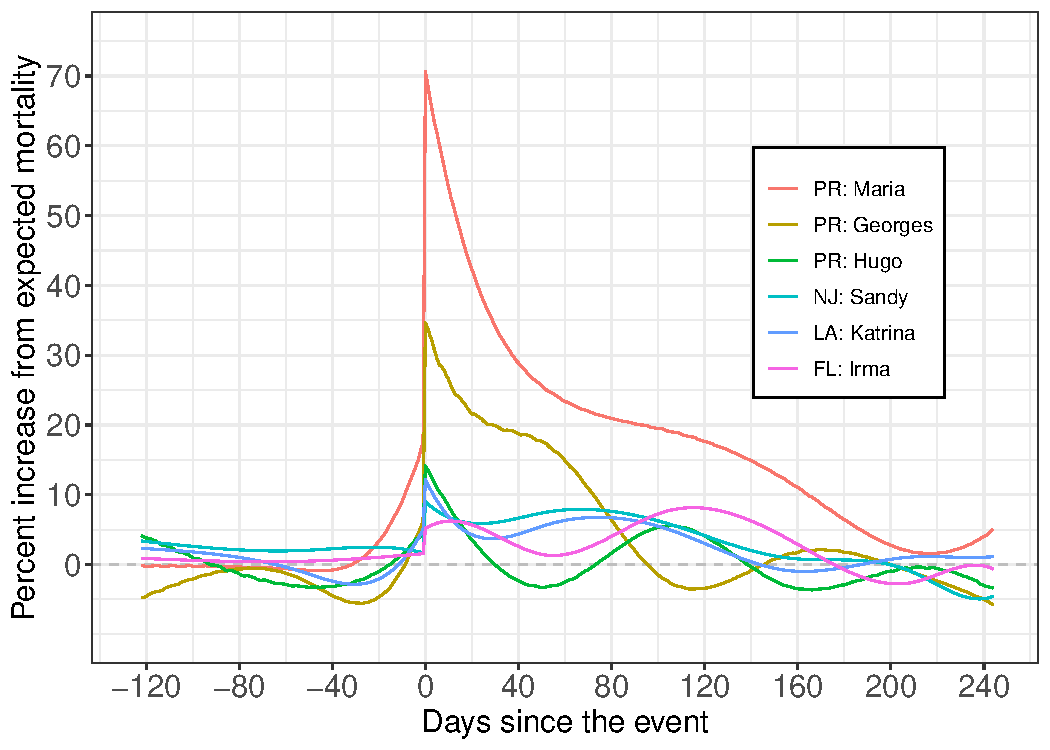
\includegraphics[width=1\linewidth]{figs/figure-1a.pdf} 
	\end{subfigure}&
	\begin{subfigure}[t]{0.30\linewidth}
		\centering
		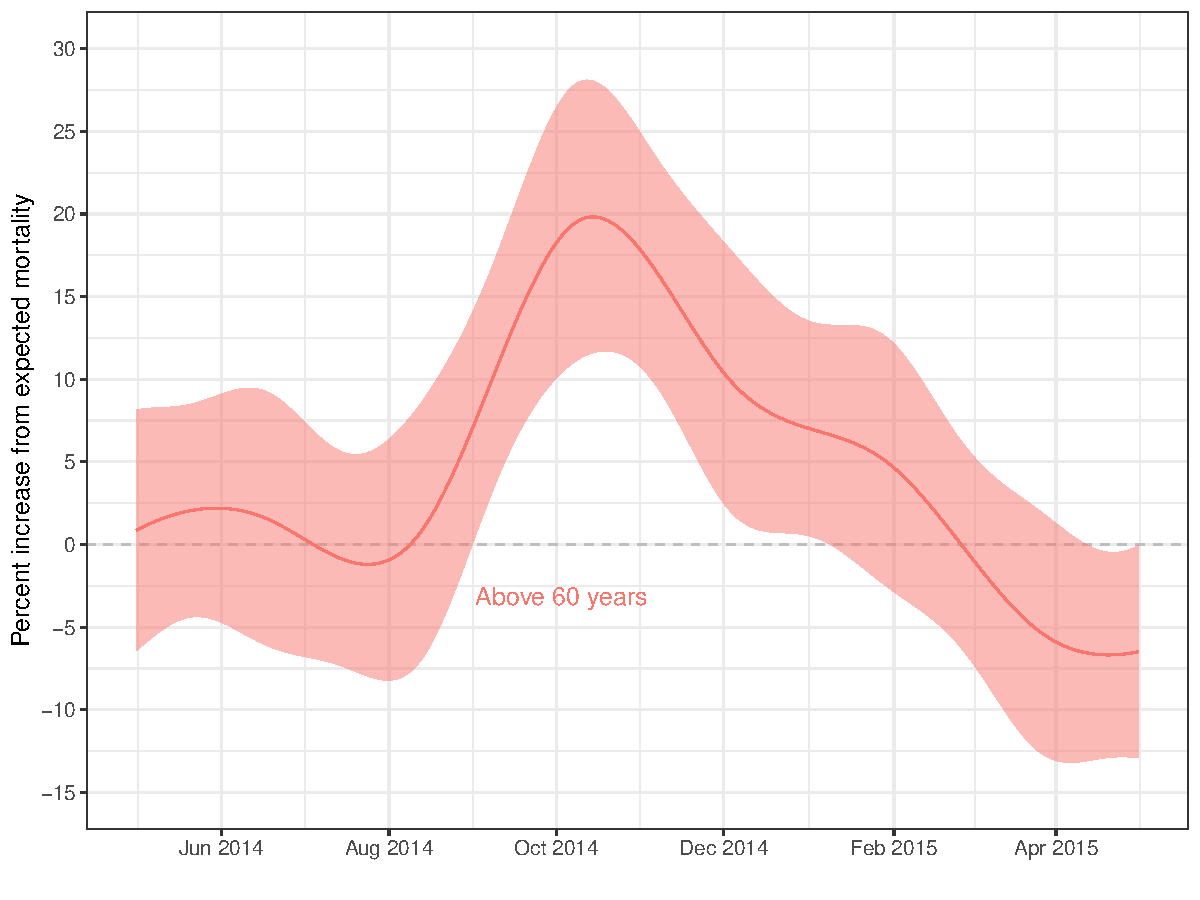
\includegraphics[width=1\linewidth]{figs/figure-1b.pdf}
	\end{subfigure}&
	\begin{subfigure}[t]{0.30\linewidth}
		\centering
		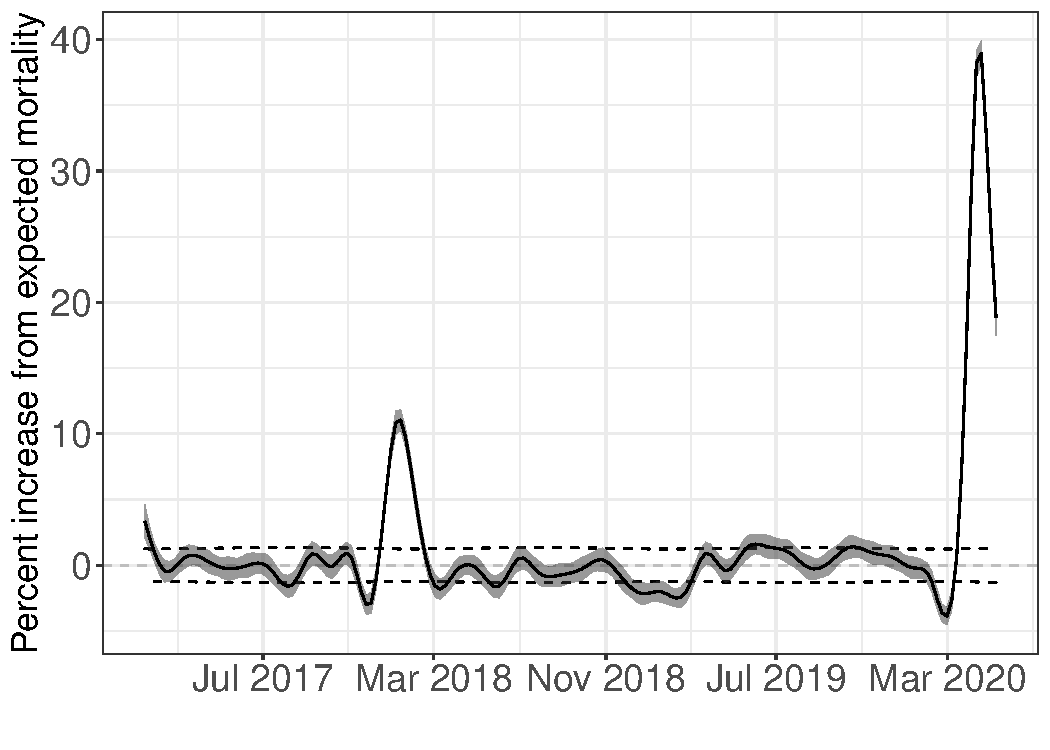
\includegraphics[width=1\linewidth]{figs/figure-1c.pdf}
	\end{subfigure}\\
    \end{tabular}
    \caption{Estimated event effects as percent increase over expected mortality. A) Comparison of six hurricanes. B) Estimated increase and point-wise confidence intervals  during the Chikungunya epidemic in Puerto Rico. C) Estimated increase and confidence interval for the the United States from January 2017 through May 2020.}
    \label{fig:fhat-estimates}
\end{figure}

\subsection{Quantifying the effects of epidemics}
\label{subsec:epidemics}
Our approach can also be used to detect and quantify the effects of epidemics or outbreaks. As an example, we fit our model to Puerto Rico mortality data from 1985 to 2020 and, apart from the hurricane seasons mentioned in the previous section, we detected an unusual increase in mortality rates from July 2014 to February 2015. These period coincide with the 2014-2015 Chikungunya outbreak \cite{sharp2016surveillance, hsu2019risk}  (Figure \ref{fig:fhat-estimates}B). The effects were particularly strong on individuals over 60 years and for the 0 to 4 years age group. (Supplemental Figure  \ref{supp-fig:chikungunya-agegroups}).

Although mortality records for the time period of the COVID-19 pandemic are not yet complete, the Center for Disease Control and Prevention (CDC) has implemented a correction to the most recent counts and are making weekly state-level data from January 2017 to May 12, 2020 publicly available \cite{cdc2020covid19}. We fit our model to these data for each state and our event effect estimates clearly detect the COVID-19 pandemic for several states, as well as the 2018 flu epidemics (Supplemental Figure \ref{supp-fig:covid19-states}). By aggregating the results for the entire United States we confirm that the COVID-19 pandemic had a substantially larger impact than the 2018 flu season
(Figure \ref{fig:fhat-estimates}C).
 
\subsection{Excess mortality estimates}
\label{subsec:excess-mortality}
Once we have fit our model, we can compute excess mortality estimates for any time period as well as standard errors that take into account, not just sample variability associated with count processes, but natural variation as well. We used the estimated parameters from the Puerto Rico data to compute excess deaths for the 365 days following the day hurricanes Georges, and Mar\'ia made landfall. We also computed these quantities for the 365 days following the start of the detected effects from the 2014 Chikungunya outbreak. Finally, we computed excess deaths in Puerto Rico during the COVID-19 pandemic, specifically from March 1, 2020 to April 15 2020, the last day for which the death registry has complete data (typically, it takes 90 days for 99\% of deaths to be registered). 

For Mar\'ia the excess death curve grew for over six months after landfall, with a point estimate on March 20, 2018, six months after landfall, of 3,229 (95\% CI: 2,794 to 3,664), and for Georges the excess death curve grew for over three months after landfall, with a point estimate on December 21, 1998, three months after landfall, of 1,232 (95\% CI: 945 to 1,519) (Figure \ref{fig:excess-deaths}A). The period of July 14, 2014 to February 20, 2015, associated with a Chikungunya outbreak was also identified to have unusually high mortality rates. However, we also noted a decrease in cumulative deaths for several months after the February 20 consistent with a \emph{harvesting effect} \cite{hajat2005mortality, dushoff2006mortality}. A year after the start of the Chikungunya epidemic, on July 14, 2015 we observe a point estimate for excess mortality of 975 (95\% CI:395 to 1,556) (Figure \ref{fig:excess-deaths}A). We note that for the period of March 15, 2020 to April 15, 2020, associated with the COVID-19 pandemic, we do not observe an effect as nearly as large as for these other three events.

\begin{figure}[ht]
	\begin{tabular}{lll}
	A&B&C\\
	\begin{subfigure}[t]{0.3\linewidth}
		\centering
		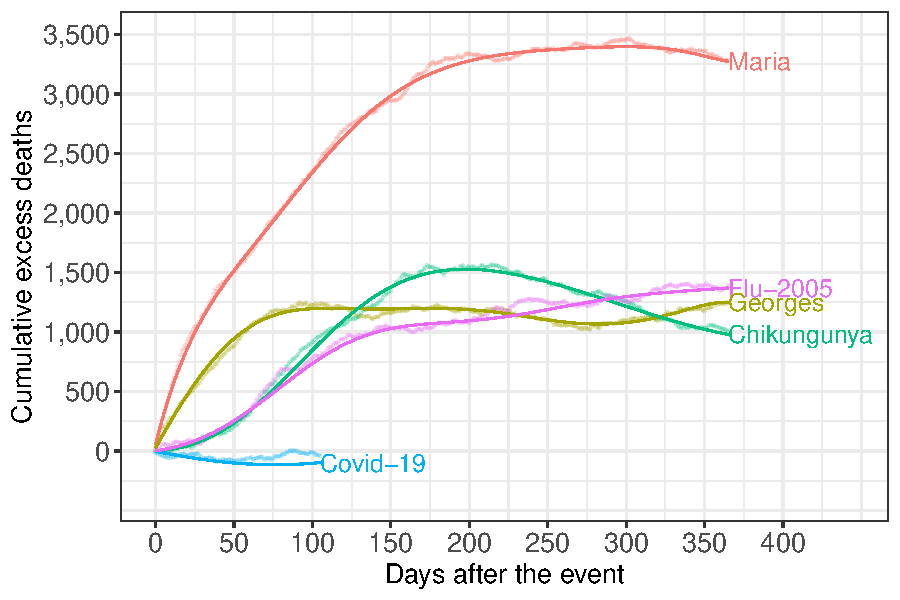
\includegraphics[width=1\linewidth]{figs/figure-2a.pdf} 
	\end{subfigure}&
	\begin{subfigure}[t]{0.3\linewidth}
		\centering
		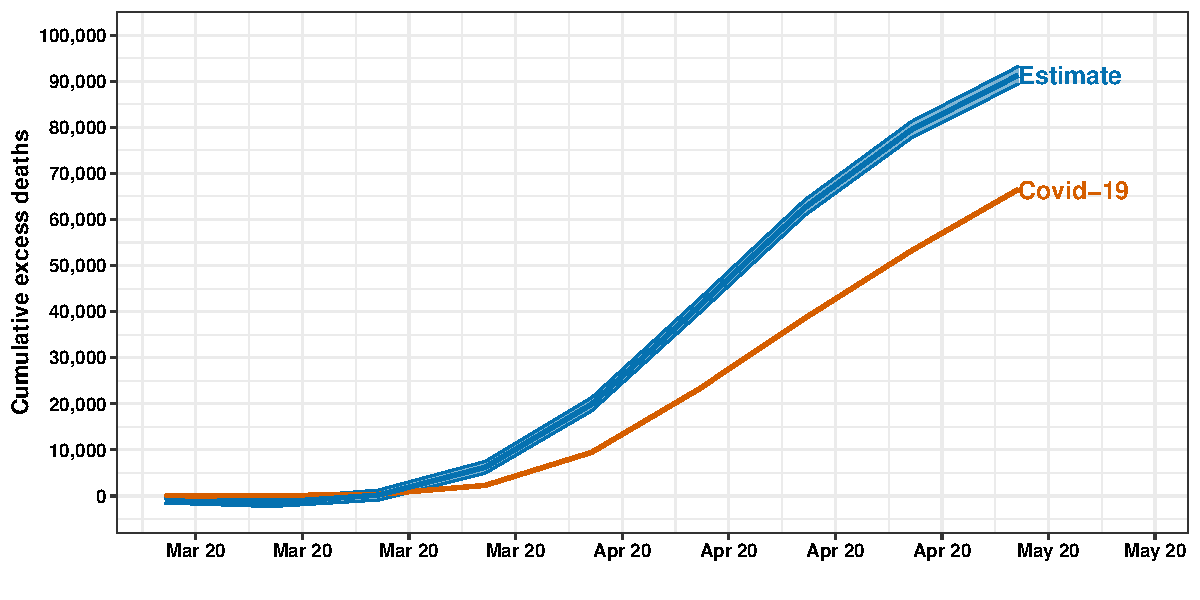
\includegraphics[width=1\linewidth]{figs/figure-2b.pdf}
	\end{subfigure}&
	\begin{subfigure}[t]{0.3\linewidth}
		\centering
		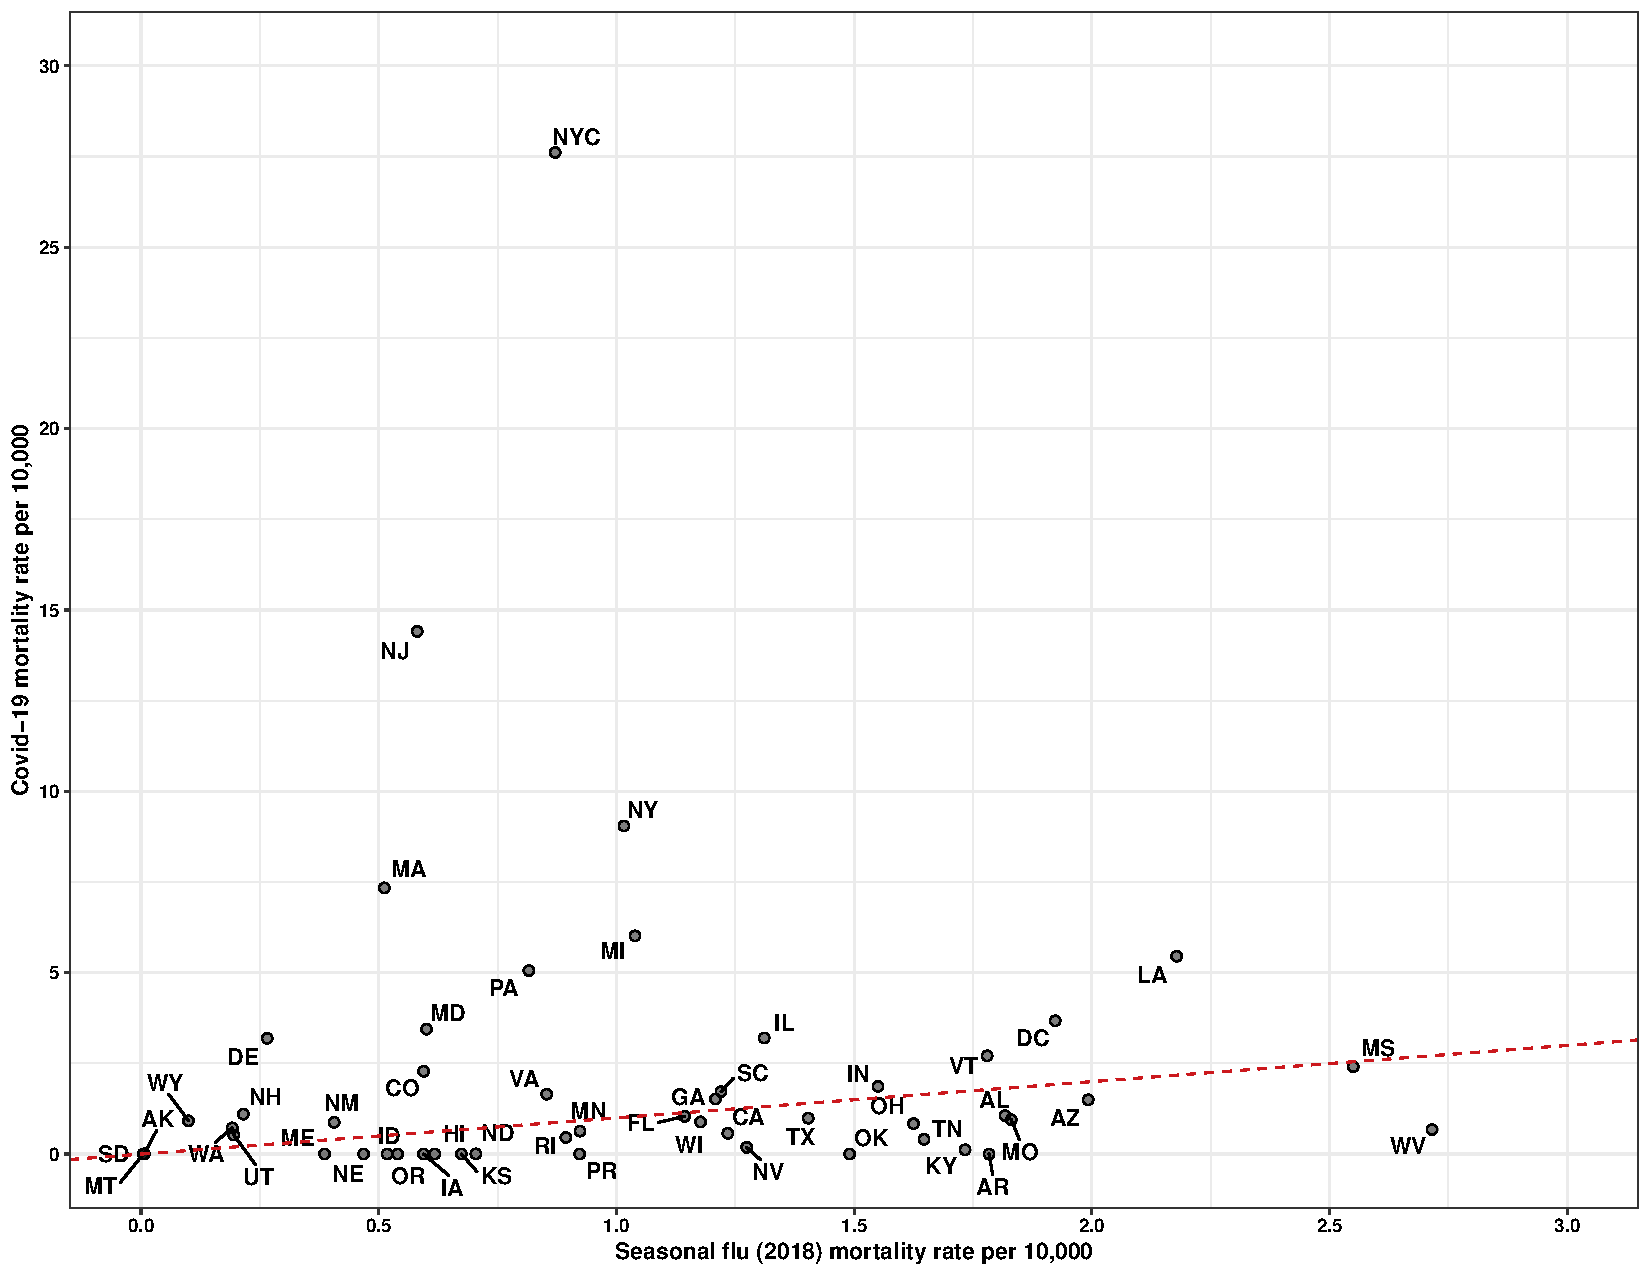
\includegraphics[width=1\linewidth]{figs/figure-2c.pdf}
	\end{subfigure}\\
	\end{tabular}
    \caption{Cumulative excess mortality estimates. A) Daily excess death estimates and 95\% confidence intervals for events in Puerto Rico starting on September 20, 2017, September 21, 1998, July 14, 2014, and March 1, 2020 for Hurricane Mar\'ia, Hurricane Georges, the Chikungunya epidemic, and the COVID-19 pandemic, respectively.  B) Estimated cumulative excess mortality and reported COVID-19 cumulative deaths in the United States. C) State-specific cumulative excess death estimates from March 1, 2020 to May 9, 2020, the period associated with the COVID-19 pandemic, plotted against the excess mortality estimates from December 10, 2017 to February 17, 2018, the period associated with the 2018 flu season. The identity line is represented in red and separates states in which the increase in mortality was higher during COVID-19 from those in which the increase in mortality was higher during the 2018 flu season.}
    \label{fig:excess-deaths}
\end{figure}

Next, using the CDC data we computed excess mortality for the period of the COVID-19 pandemic for which we have data, specifically for the week ending on March 15, 2020 to the week ending on May 9, 2020. When we compared these numbers to the reported numbers of COVID-19 deaths \cite{smith2020coronavirus}, we find a difference of 29,246 (95\% CI: 27,317 to 31,175) deaths (Figure \ref{fig:excess-deaths}B, Table \ref{tab:covid19-states}). We also note that in the US, the number of excess deaths during the COVID-19 pandemic are much larger than the 2018 flu season, although this is not true for all states (Figure \ref{fig:excess-deaths}C, Table \ref{tab:covid19-states}). We also note that 58\% of the cases come from the four northeast states: New York, New Jersey, Massachusetts, and Pennsylvania (Supplemental Figure \ref{supp-fig:covid19-states}). We note that Connecticut was not included in the analysis due to missing data.

\begin{table}
\centering
\tiny
\begin{tabular}{|l|lll|ll|}
  \hline
 & \multicolumn{3}{c|}{COVID-19} & \multicolumn{2}{c|}{2018 Flu} \\
\hline
State & Excess & Reported & Rate  & Excess & Rate \\
 & mortality (SD) & cases & (per million) & mortality (SD) & (per million) \\
\hline
New York City & 24132 (134) & 19324 & 2873 & 806 (129) & 96 \\ 
  New Jersey & 13364 (153) & 9116 & 1505 & 525 (147) & 59 \\ 
  New York (not including NYC) & 11178 (179) & 7260 & 1011 & 1147 (174) & 104 \\ 
  Massachusetts & 5995 (131) & 4840 & 870 & 325 (126) & 47 \\ 
  Michigan & 6240 (189) & 4526 & 625 & 1025 (187) & 103 \\ 
  Pennsylvania & 7638 (214) & 3793 & 597 & 1022 (206) & 80 \\ 
  Louisiana & 2544 (133) & 2267 & 547 & 1053 (129) & 226 \\ 
  District of Columbia & 309 (37) & 311 & 437 & 116 (36) & 165 \\ 
  Maryland & 2632 (120) & 1614 & 435 & 355 (117) & 59 \\ 
  Illinois & 4802 (205) & 3362 & 379 & 1601 (199) & 126 \\ 
  Vermont & 212 (41) & 53 & 340 & 106 (40) & 169 \\ 
  Delaware & 283 (49) & 221 & 291 & 58 (47) & 60 \\ 
  Colorado & 1588 (91) & 965 & 276 & 307 (91) & 53 \\ 
  Mississippi & 791 (94) & 421 & 266 & 773 (92) & 260 \\ 
  Virginia & 2147 (132) & 827 & 252 & 671 (131) & 79 \\ 
  South Carolina & 1265 (115) & 330 & 246 & 667 (113) & 129 \\ 
  Indiana & 1646 (144) & 1490 & 244 & 898 (141) & 133 \\ 
  Arizona & 1467 (156) & 532 & 202 & 1390 (157) & 191 \\ 
  New Hampshire & 255 (54) & 131 & 188 & 45 (53) & 33 \\ 
  Ohio & 1958 (233) & 1331 & 168 & 1724 (226) & 147 \\ 
  New Mexico & 345 (73) & 191 & 164 & 54 (73) & 26 \\ 
  Georgia & 1599 (201) & 1380 & 151 & 1398 (197) & 132 \\ 
  Rhode Island & 152 (50) & 418 & 144 & 81 (50) & 77 \\ 
  Minnesota & 781 (119) & 558 & 139 & 478 (118) & 85 \\ 
  Florida & 2854 (372) & 1714 & 133 & 2458 (368) & 114 \\ 
  Texas & 3840 (370) & 1086 & 132 & 4021 (359) & 139 \\ 
  Wisconsin & 715 (133) & 398 & 123 & 653 (131) & 112 \\ 
  Missouri & 736 (169) & 492 & 120 & 1169 (164) & 191 \\ 
  Washington & 711 (168) & 925 & 93 & -13 (164) & -2 \\ 
  Alabama & 400 (129) & 390 & 82 & 904 (126) & 184 \\ 
  California & 2975 (501) & 2732 & 75 & 4530 (487) & 115 \\ 
  Tennessee & 481 (172) & 241 & 70 & 1120 (169) & 164 \\ 
  Utah & 213 (62) & 66 & 66 & 47 (62) & 15 \\ 
  Nevada & 187 (77) & 306 & 61 & 290 (76) & 94 \\ 
  Kentucky & 231 (113) & 312 & 52 & 708 (111) & 158 \\ 
  Arkansas & 129 (94) & 88 & 43 & 537 (92) & 178 \\ 
  Iowa & 136 (91) & 252 & 43 & 160 (89) & 51 \\ 
  Oregon & 120 (112) & 127 & 29 & 47 (111) & 11 \\ 
  South Dakota & 25 (47) & 34 & 29 & -56 (47) & -63 \\ 
  Kansas & 66 (80) & 172 & 23 & 230 (79) & 79 \\ 
  Maine & 27 (54) & 64 & 20 & 46 (54) & 34 \\ 
  Idaho & 33 (53) & 67 & 19 & 97 (54) & 54 \\ 
  Nebraska & 37 (66) & 95 & 19 & 50 (64) & 26 \\ 
  Wyoming & 9 (30) & 7 & 16 & 15 (31) & 26 \\ 
  Montana & -7 (49) & 16 & -6 & -72 (48) & -68 \\ 
  Alaska & -34 (32) & 8 & -47 & -6 (33) & -9 \\ 
  Hawaii & -81 (51) & 17 & -57 & 87 (51) & 62 \\ 
  North Dakota & -88 (41) & 35 & -115 & 18 (42) & 24 \\ 
 \hline
  Total & 107041 (1091) & 74905 & 347 & 33664 (1066) & 109 \\ 
  \hline
 \end{tabular}
 \caption{Excess mortality estimates for the weeks ending on March 14, 2020 to May 9, 2020 (COVID-19) and  December 10, 2017 to February 17, 2018 (2018 Flu). The standard deviation for excess mortality for these periods is included in parenthesis. The states are ordered by the per-million excess mortality rate. Connecticut and North Carolina are excluded due to missing data. Numbers for New York do not include New York City which is listed separately.}
 \label{tab:covid19-states}
 \normalsize
\end{table}
 
 

\subsection{Across group comparisons}
\label{subsec:group-comparison}
Since our model provides both estimates and standard errors of event effects, we can compare the effects for two or more groups and assess the statistical significance of the observed differences. We demonstrate how this can be used by comparing black and white populations during the COVID-19 pandemic in Cook County, Illinois. At the time of writing, the Cook County Medical Examiner's Office was making up-to-date records available online including demographic information for each individual. This office investigates any human death in Cook County that falls within categories such as criminal violence, suicide, accident, diseases constituting a threat to public health, among other unusual circumstances \cite{cookcovid19}. If we consider $\mu_t$ to be the expected number of deaths recorded by the Medical Examiner's Office, we can fit our model and interpret $f(t)$ as the percent increase in deaths examined by this office. We fit the model to these data and clearly observed the effects of the COVID-19 epidemic, in particular among individuals over 75. However, a persistent increase in mortality above normal levels is observed for individuals above 40 (Supplemental Figure \ref{supp-fig:cook-agegroups}).  Furthermore, we found a difference in the effect  between white and black individuals in the months of March and April (Figure \ref{fig:cook-white-v-black}). Among those between 40 and 59 years of age, the percent increase in medical examiner death rates for Cook county was as high as 185\% (95\% CI: 144\% to 227\%) and 57\% (95\% CI:24\% to 89\%) on April 11 for blacks and whites, respectively. Furthermore, for the 60 to 74 age group we observed a percent increase of 
600\% (95\% CI: 525\% to 674\%) and 480\% (95\% CI: 416\% to 543\%) on April 25, respectively. Finally, the percent increase for individuals 75 years and older was 2,282\% (95\% CI: 2,047\% to 2,518\%) and 1,222\% (95\% CI: 1,109\% to 1,335\%) on April 29, respectively, another statistically significant finding (Figure \ref{fig:cook-white-v-black}).  The population size, in this database, for other racial groups was substantially smaller and were not included in the analysis.

\begin{figure}[ht]
	\begin{tabular}{lll}
	A&B&C\\
	\begin{subfigure}[t]{0.3\linewidth}
		\centering
		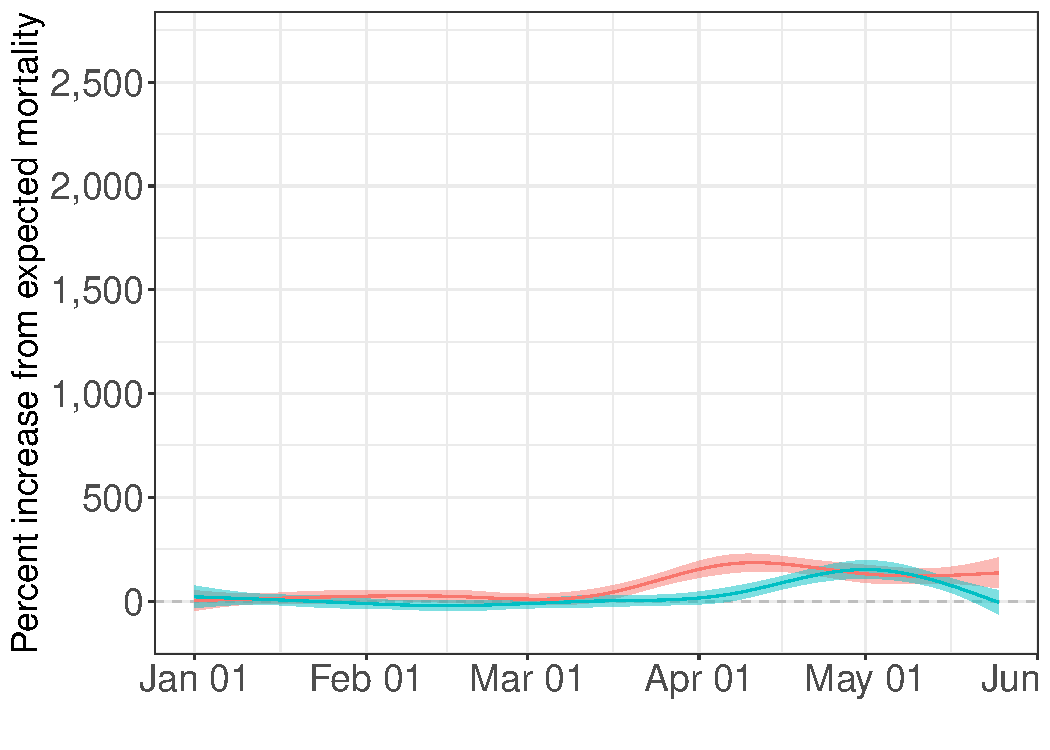
\includegraphics[width=1\linewidth]{figs/figure-3a.pdf} 
	\end{subfigure}&
	\begin{subfigure}[t]{0.3\linewidth}
		\centering
		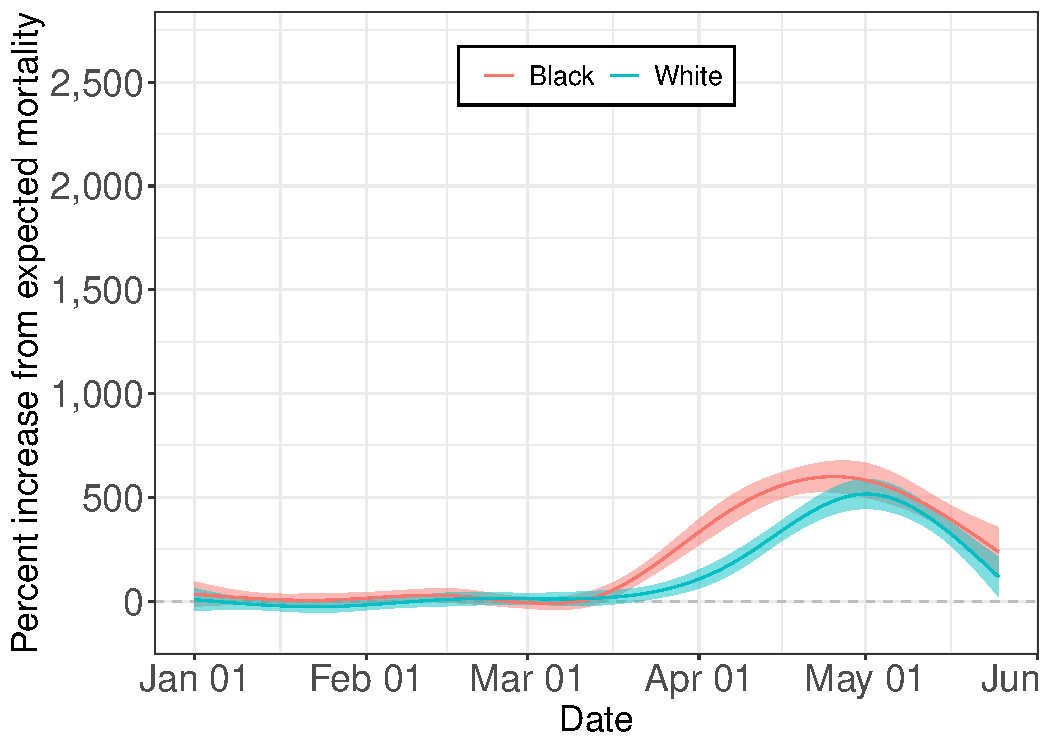
\includegraphics[width=1\linewidth]{figs/figure-3b.pdf}
	\end{subfigure}&
	\begin{subfigure}[t]{0.3\linewidth}
		\centering
		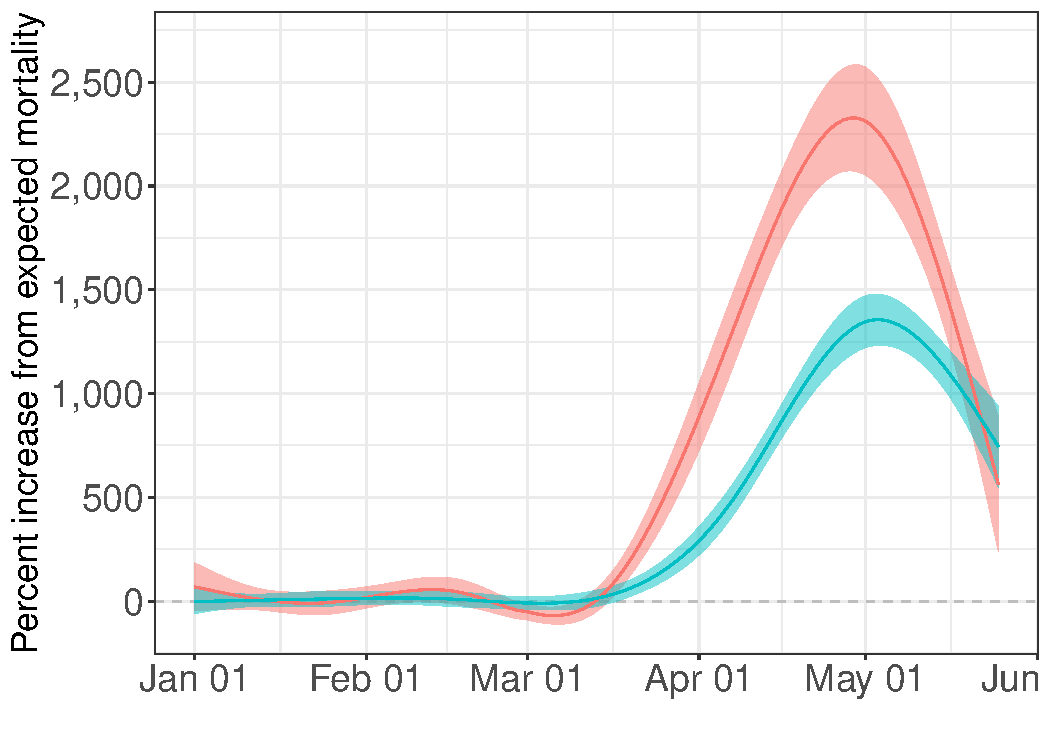
\includegraphics[width=1\linewidth]{figs/figure-3c.pdf}
	\end{subfigure}\\
	\end{tabular}
	\caption{Comparison of estimated percent increase in mortality in Cook county, Illinois, for individuals above 40 between whites and blacks with corresponding 95\% confidence intervals. A) 40 to 59 age group. B) 60 to 74 age group. C) 75 and over age group.}
	\label{fig:cook-white-v-black}
\end{figure}



\subsection{Natural Variability and Correlated Counts}
\label{subsec:natural-variability}
Exploration data analysis after fitting a standard Poisson model demonstrates that the daily data measurements are correlated (Supplemental Figure \ref{supp-fig:correlated-errors}). Assuming independence, when in fact variables are correlated, leads to underestimates of the standard error of sums or averages. Cumulative excess mortality is the sum of excess deaths during a period of interest, therefore accounting for correlation allows our approach to better estimate the uncertainty of this quantity. To demonstrate this, we compared our model to a standard Poisson model and a over-dispersed Poisson model both assuming independent outcomes \cite{farrington1996statistical,hohle2008count,noufaily2013improved,salmon2016monitoring}. We fit each of the three models to the Puerto Rico data for individuals 75 and over, and randomly selected 100 intervals of sizes $L$ = 10, 50, and 100 days from periods with no events and computed the total number of deaths in each interval $S_l = \sum_{t \in L} Y_t$. We then used the fitted models to estimate the expected value $\hat{\mbox{E}}(S_l)$ and standard error  and $\hat{\mbox{SE}}(S_l)$ and form a z-statistic $Z_l = [S_l - \hat{\mbox{E}}(S_l)]/\hat{\mbox{SE}}(S_l)$. The Central Limit Theorem predicts that, if the expected value and standard errors are estimated correctly, $Z_l$ is approximately normal with expected value 0 and standard error 1. We found that the Poisson and over-dispersed Poisson model underestimate the variance of this sum, while modeling the correction improves our standard error estimates (Figure \ref{fig:deaths-qqplots}). 
 
\begin{figure}[ht]
	\begin{tabular}{lll}
	A&B&C\\
	\begin{subfigure}[t]{0.3\linewidth}
		\centering
		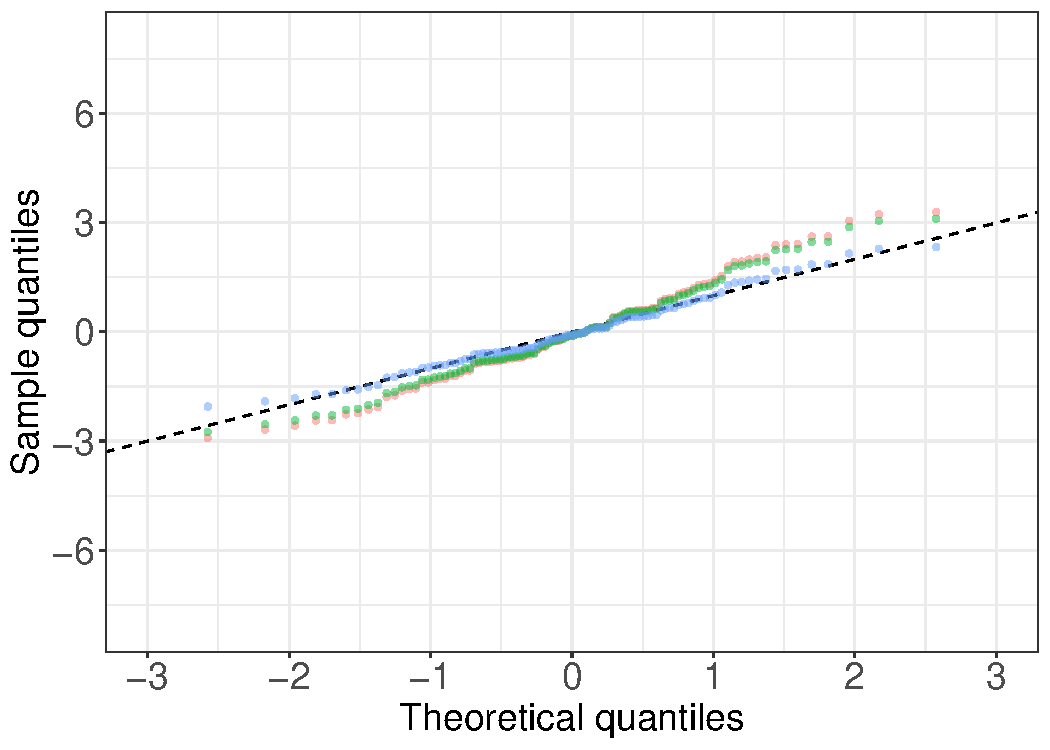
\includegraphics[width=1\linewidth]{figs/figure-5a.pdf} 
	\end{subfigure}&
	\begin{subfigure}[t]{0.3\linewidth}
		\centering
		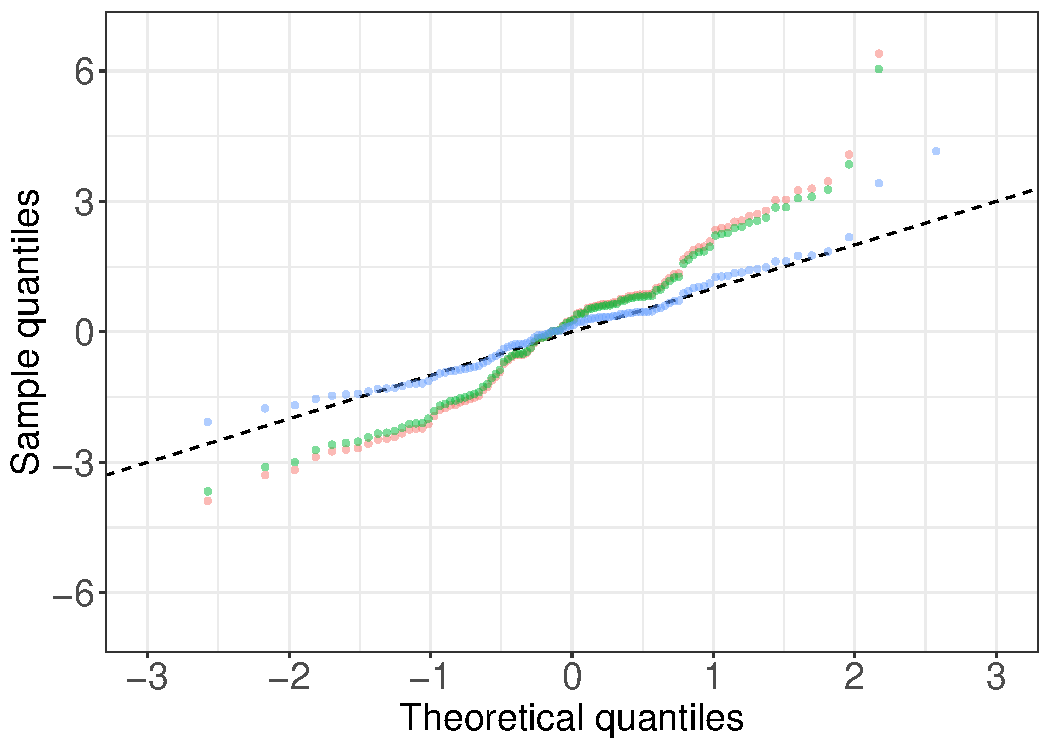
\includegraphics[width=1\linewidth]{figs/figure-5b.pdf}
	\end{subfigure}&
	\begin{subfigure}[t]{0.3\linewidth}
		\centering
		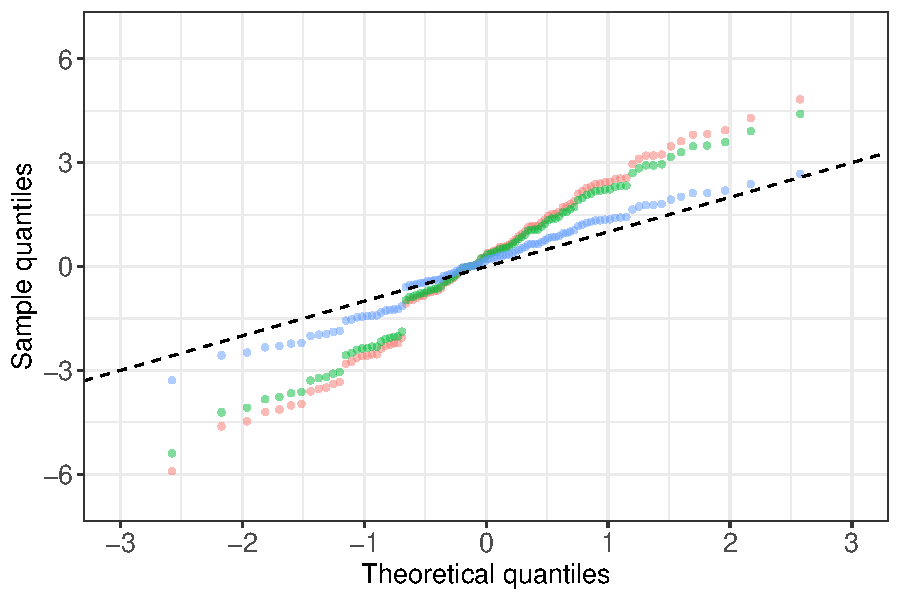
\includegraphics[width=1\linewidth]{figs/figure-5c.pdf}
	\end{subfigure}\\
	\end{tabular}
	\caption{Accounting for correlation in the error structure improves uncertainty estimates. We fitted our model along with a Poisson and over-dispersed Poisson GLM to Puerto Rico data of individuals 75 years and over, and randomly picked 100 intervals of varying sizes to compute z-scores of total number of deaths. Each plot shows the Pearson residual quantiles versus theoretical quantiles from the standard normal distribution. A) Intervals of 10 days. B) Intervals of 50 days. C) Intervals of 100 days.}
	\label{fig:deaths-qqplots}
\end{figure}

\subsection{An index based on relative proportion of specific causes of death}
\label{subsec:causes-deaths}

Limitations of our approaches for detecting and monitoring health crises in real-time are that it requires 1) complete death count data and 2) an estimate of population displacement. Note that incomplete death counts or underestimates of population displacement will result in an underestimate of the death rate. However, if we redefine $Y_t$ as the number of deaths due to a specific cause at time $t$ and $N_t$ as the total number of recorded deaths at time $t$, then the estimate of $f$ can be interpreted as the percent increase in the proportion of deaths due to that cause, even if the data is incomplete. The underlying cause of death for the Puerto Rico mortality data was coded using the tenth version of the International Classifications of Diseases (ICD10) codes \cite{world2004icd}. Because deaths due to bacterial infections have been reported to increase after natural disasters in locations with poor public health infrastructure \cite{ligon2006infectious, cook200810th}, we defined an index based on ICD10 codes between A00 and A79 as bacterial infections. We found that deaths attributable to this cause were elevated after the landfall of hurricane Mar\'ia in Puerto Rico (Figure \ref{fig:mortality-index}A) pointing the possibility that this index could be used in real-time to detect challenges to the health system. During the COVID-19 pandemic, if under-reporting is occurring, one would expect causes related to the respiratory system to increase. A similar index for respiratory diseases defined as ICD10 codes between J00 and J99 computed for the COVID-19 pandemic shows no anomalies  (Figure \ref{fig:mortality-index}B).

\begin{figure}[ht]
	\begin{tabular}{lll}
	A&B\\
	\begin{subfigure}[t]{0.49\linewidth}
		\centering
		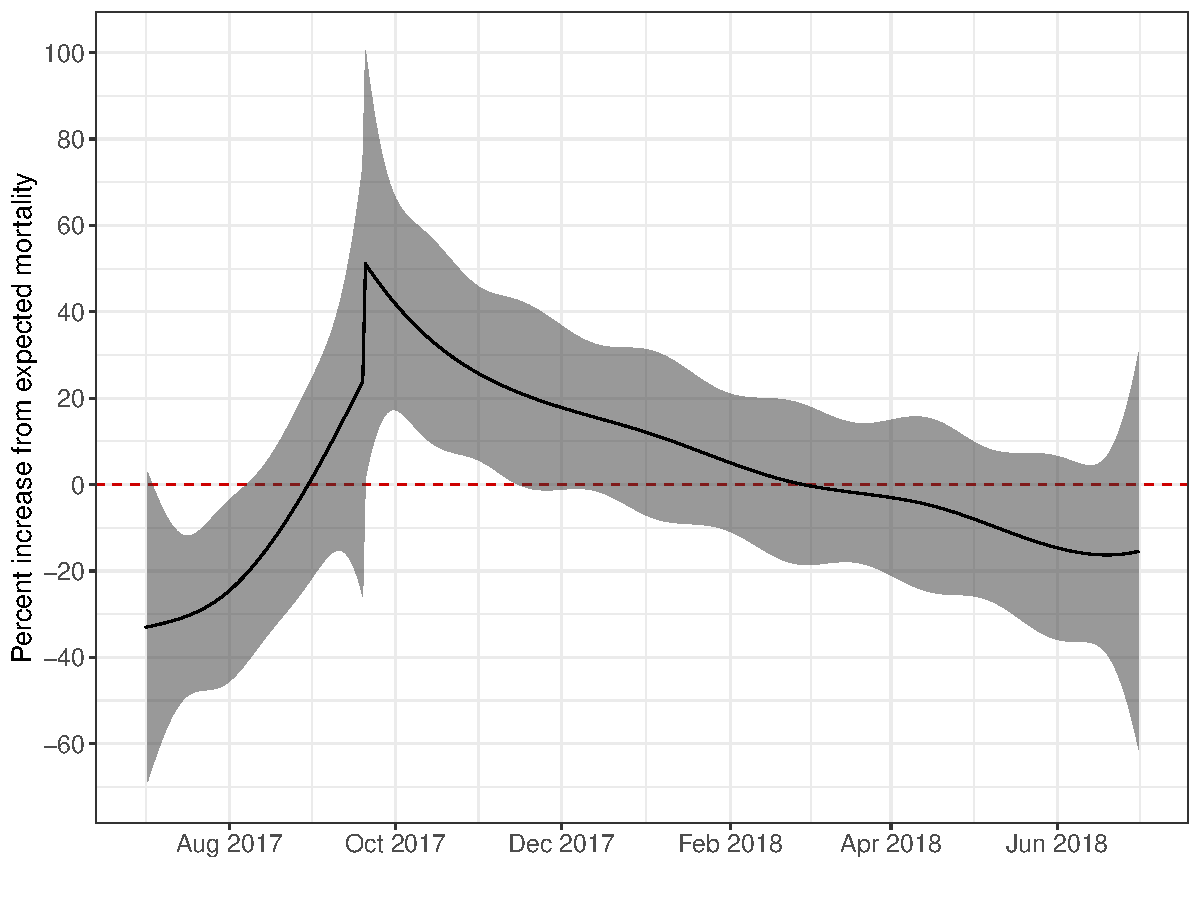
\includegraphics[width=1\linewidth]{figs/figure-4a.pdf} 
	\end{subfigure}&
	\begin{subfigure}[t]{0.49\linewidth}
		\centering
		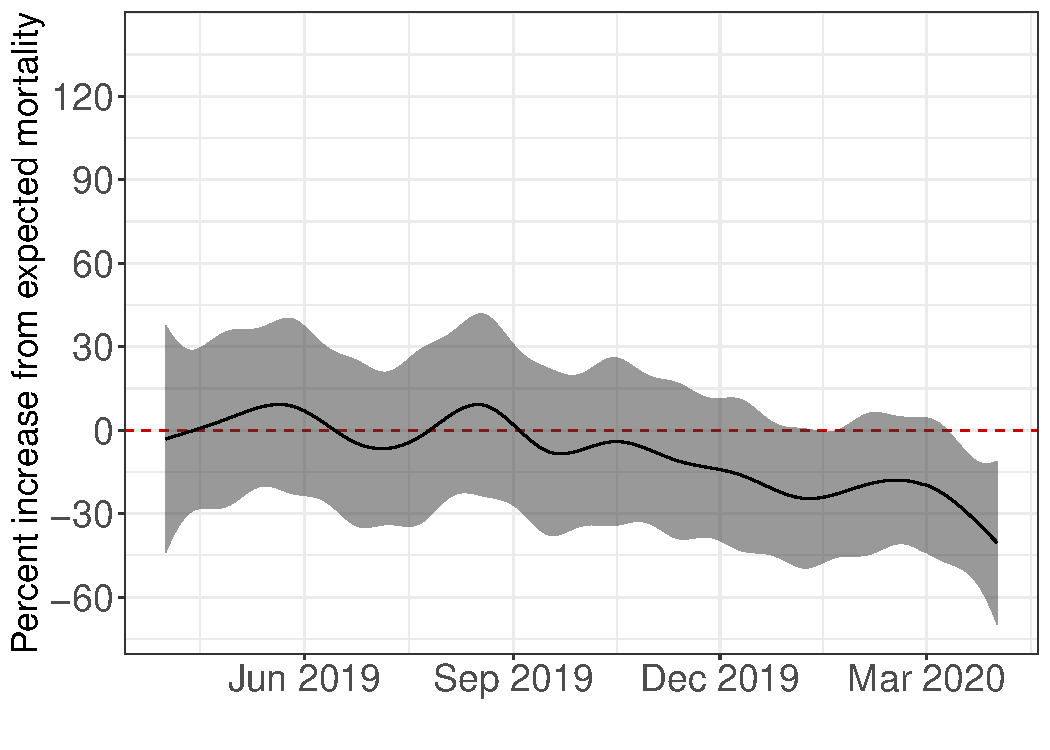
\includegraphics[width=1\linewidth]{figs/figure-4b.pdf}
	\end{subfigure}&\\
    \end{tabular}
	\caption{Cause-specific mortality index. The solid-black line corresponds to the percent change in proportion of mortality, $\hat{f}(t)$, attributable to a cause of interest. The shaded area represents a 95\% confidence interval for $\hat{f}(t)$. A) Bacterial infections mortality index defined as ICD10 codes between A00 and A79 for the dates around Hurricane Mar\'ia. B) Respiratory diseases mortality index defined as ICD10 codes between J00 and J99 for the dates around the COVID-19 pandemic in Puerto Rico.}
	\label{fig:mortality-index}
\end{figure}


\section{Methods}
\label{sec:methods}

In this section we provided a description of the model and estimation procedure applied to obtain results. All details of our analysis are available by examining the code which is made available on GitHub: \url{https://github.com/rafalab/excess-mortality-paper}
The code for the R package implementing the methods is also available on GitHub: \url{https://github.com/rafalab/excessmort}

\subsection{Mortality Data}
\label{subsec:mortality-data}
We obtained detailed mortality and population size data related to hurricanes Hugo, Georges, and Mar\'ia in Puerto Rico, Katrina in Louisiana, Sandy in New Jersey, and Irma in Florida. For Puerto Rico, we requested individual level mortality information with no personal identifiers from the Department of Health of Puerto Rico and obtained individual records including date, gender, age, and cause of death from January 1985 to May 2020. We used this data to construct daily death counts for different strata of the Puerto Rican population throughout the study period. We also obtained daily death counts from Florida, New Jersey, and Louisiana’s Vital Statistic systems from January 2015 to December 2018, January 2007 to December 2015, and January 2003 to December 2006, respectively. Note that we did not obtain individual records from these jurisdictions. We also obtained mortality data made public on May 29, 2020 by the CDC  \cite{cdc2020covid19}. This dataset included weekly estimates of death counts for each state and Puerto Rico for the period of January 2017 and May 2020. 
Finally, we obtained individual level mortality data from the Cook County, IL, medical examiner office \cite{cookcovid19}. These data included demographic information for each death including age, sex, and race.

\subsection{Population Estimates}
\label{subsec:population}
Yearly population estimates for Puerto Rico were obtained from the Puerto Rico Statistical Institute. Yearly population estimates for other US states were obtained from the US Census bureau. We computed daily population estimates via linear interpolation of the available data. To obtain an estimate of the population displacement after Hurricane Mar\'ia in Puerto Rico, we use population proportion estimates from Teralytics. Teralytics is a company that works with governments and private clients to assess human movement by partnering with mobile network operators. This company provided daily population proportion estimates relative to an undisclosed baseline from May 31, 2017 to April 30, 2018. This was based on all subscribers of a major, undisclosed, telecommunications company in Puerto Rico. Due to structural damage post Hurricane Maria, proportion estimates for the four weeks after the storm were not provided. We imputed missing data with linear interpolation of observed values. We then computed population estimates by multiplying the US census population estimate on July 19, 2017, Teralytics baseline date, times the aforementioned proportions, and obtained smooth values using local regression (Supplemental Figure \ref{supp-fig:pop-displacement-pr}).

\subsection{Statistical model}
\label{subsec:statistical-model}
We assume the mortality counts at $t$ follows a generalized linear mixed model defined in Section  \ref{subsec:model-based}. Specifically, we assume:
\begin{equation*}
    Y_t \mid \varepsilon_t \propto \mbox{Poisson}\left\{ \mu_t 
    \left[1 + f(t)\right]  \varepsilon_t \right\}, \mbox{ for } t = 1, \dots,T 
\end{equation*}
where the expected counts have the form:
\begin{equation*}
    \mu_t =N_t  \exp[\alpha(t) + s(t) + w(t)]
\end{equation*}
and the vector $[\varepsilon_1, \ldots, \varepsilon_T]^\top$ follows a multivariate normal distribution with mean 1 and variance-covariance matrix $\Sigma$ determined by an auto-regressive (AR) process of order $p$:
\begin{equation*}
    \Sigma = \sigma^2
    \begin{pmatrix} 1 & \rho_1 & \rho_{2} & \dots & \rho_{T} \\ 
    \rho_{1} & 1 & \rho_{1} & \ldots & \rho_{T-1} \\
    \vdots & \vdots & \vdots & \vdots & \vdots \\
    \rho_{T} & \rho_{T-1} & \rho_{T-2} & \dots & 1 \\ 
    \end{pmatrix}.
\end{equation*}
Here $\sigma$ corresponds to the standard deviation associated with natural variability and $\rho_h$ is the auto-correlation of two error terms that are $h$ time units from each other. In practice, obtaining Maximum Likelihood Estimates (MLE) for this model is not straight-forward, in particular because the flexibility in $f(t)$ and $\Sigma$ makes the model non-identifiable in practice. To overcome this challenge, we implemented a three step approach that works well in practice, as demonstrated both by simulation and empirical validation.

We start by modeling the yearly trend $\alpha(t)$ with natural cubic splines with a knot every seven years. We model the seasonal effect $s(t)$ with a harmonic model with 2 harmonics. Finally, $w(t)$
represents seven parameters, one for each day of the week. 

Natural disasters and outbreaks are rare, hence we assume that for the majority of time points $f(t)$ is 0, which implies that 
\begin{equation*}
    Y_t \mid \varepsilon_t \propto \mbox{Poisson}(\mu_t  \varepsilon_t )
\end{equation*}
and that, for example, for $N = T / 365$ years of daily data we would have $T$ data points to fit a model with at most N/7 + 7 + 4 + 1 parameters. For seven years of data this translates into 2,556 data points and 13 parameters. As a result, we can obtain highly precise estimates even in the presence of the extra dispersion introduced by $\varepsilon$. We therefore fit a Poisson Generalized Linear Model (GLM) to regions that we know do not include natural disasters or outbreaks and in the next step consider the MLE, $\hat{\alpha}(t)$, $\hat{s}(t)$, and $\hat{w}(t)$ as fixed.

In the second step we estimate $\Sigma$, and to do this we select a control contiguous region for which we know $f(t)=0$. To estimate the $\sigma^2$ and the autoregressive parameters we can use the law of total variance to note that the observed percent change from the mean
\begin{equation*}
    r_t = \frac{Y_t - \mu_t}{\mu_t}
\end{equation*}
has expected value and variance
\begin{equation*}
    \mathbb{E}\left(r_t \right) = 0 \mbox{ and } \mbox{Var}\left(r_t\right)= \sigma^2 + 1/\mu_t
\end{equation*}
Intuitively, these two components are the variance added by $\varepsilon$ and the Poisson variability respectively. The above implies that if we define the transformation:
\begin{equation*}
    Z_t = \frac{r_t}{\sqrt{\mbox{Var}\left(r_t\right)}}
\end{equation*}
we have an approximately normally distributed random variable with the same correlation structure as $\varepsilon_t$, which is what we want to estimate. We use the Yule-Walker equation approach to estimate the AR process parameters from the observed $Z_t$. To estimate $\sigma^2$ we use:
\begin{equation*}
    \hat{\sigma}^2 = \max\left\{ \frac{1}{T}\sum_{t=1}^T  \left(\frac{Y_t - \hat{\mu}_t}{\hat{\mu}_t}\right)^2  - \frac{1}{\mu_t}, \, 0\right\}
\end{equation*}
Using these estimates we can form an estimate $\hat{\Sigma}$ which we will consider known in the next step.

In the third step we treat $\hat{\Sigma}$ as known, assume $f(t)$ can be modeled as a natural cubic spline, and use iteratively re-weighted least squares to obtain an estimate $\hat{f}(t)$. To account for non-continuities due to direct effects from natural disasters we permit the spline to be discontinuous at the event day. 

\subsection{Approximation for uncorrelated data}
Note that our model can be easily adapted to be fitted to weekly data. In this case there is no need to include weekday effect parameters $w(t)$ and much less need for a correlation structure for the errors (Supplemental Figure \ref{supp-fig:weekly-correlated}). 

\subsection{Excess death estimates}
\label{subsec:excess-deaths}
We estimate cumulative excess deaths for any interval $I = [a, b]$ 
by adding the excess deaths for each day
in $I$: 
\begin{equation*}
    \mbox{Excess deaths} = \sum_{t = a}^b \hat{\mu}_t \hat{f}(t) 
\end{equation*}
We construct a 95\% confidence interval using the fact that the sum $\sum_{t = a}^b \hat{\mu}_t \hat{f}(t)$ is approximately normally distributed, and if we define $H$ as the \emph{hat matrix}, we can compute the variace with:
$\{ \hat{f}(a), \dots \hat{f}(b) \}^\top = H (Y_1, \dots, Y_T)^\top$ then

 \begin{equation*}
    \mbox{Var}\left[\sum_{t = a}^b \hat{\mu}_t \hat{f}(t) \right] = (\hat{\mu}_a,\dots,\hat{\mu}_b) H \hat{\Sigma} H^\top (\hat{\mu}_a,\dots,\hat{\mu}_b)^\top.
 \end{equation*}
 
\subsection{Simulation study}
\label{subsec:simulations}
To assess our procedure we conducted a Monte Carlo simulation. We start by denoting: 1) an event day, $t_0$, which may correspond to a hurricane landfall or peak-day of an epidemic, 2) an effect size, $\theta$, that represents the percent change from expected mortality at event day, and 3) a period of effect, $L$, which constitutes the number of days with unusually high levels of mortality. Second, we use a normal distribution centered at $t_0$ and scaled so that the value equals $\theta$ and that the standard deviation is equal to $L/3$ to estimate the true percent change in mortality, $f(t)$. Then we compute $\hat{\mu}_t$ for $t=1,\ldots, T$, using the Puerto Rico mortality data with model (\ref{eq:mean-model}) and generate rates $\hat{\mu}_t\left[1+f(t)\right]$. To generate the AR process, we first fit an AR model to our data and use the estimated coefficients to generate $T$ auto-correlated errors $\varepsilon_1, \dots, \varepsilon_T$. We set the standard deviation of these errors to be $\sigma = 0.05$.  Finally, we generate data $Y_t^* \sim \mbox{Poisson}\left(\hat{\mu}_t[1+f(t)][1 - \hat{\varepsilon}_t]\right)$. We generated three scenarios to mimic 1) a hurricane-like event where we expect mortality to increase rapidly and stay above normal levels for some time, 2) an epidemic-like event in which mortality increases slowly until reaching some plateau and then decreasing to normal levels, and 3) a time period of no event in which we expect our estimate of $f(t)$ to be centered around 0. For each scenario we ran 100 simulations with $t_0 = $ September 21, 1998, $\theta = 0.55$, and $L=150$ days. Our implementation produces accurate and precise results for both $f$ and $\Sigma$ (Supplemental Figure \ref{supp-fig:simulations}).

\section{Discussion}
We have introduced methods and software useful for estimating excess mortality from weekly or daily counts. The engine of our approach is a statistical model that accounts for long-term trends, seasonal effects, day of the week effects, and natural variation. An important contribution of this new approach are the improved uncertainty estimates permitted by modeling the correlation observed in the data. Another advance is the added flexibility that permits accounting for both direct and indirect effects. 

We used the model to demonstrate that the indirect effects for Hurricanes Georges and Mar\'ia on Puerto Rico were like nothing seen in previous hurricanes in the United States. We also demonstrated that the 2014 Chikungunya epidemic resulted in substantial excess mortality in Puerto Rico. These results suggest a lack of robustness of Puerto Rico's health system. We note that in New Orleans, shortly after Katrina, the U.S. Army Corps of Engineers admitted that faulty design specifications, incomplete sections, and substandard construction of levee segments, contributed to the damage and a \$14.5 billion investment was made to construct stronger levees \cite{kates2006reconstruction, interagency2007performance, adelson2018}. In contrast, after Hurricane Georges resulted in similar excess mortality toll, as far as we know, no systematic effort was put in place to improve, for example, Puerto Rico’s electrical grid nor it's data collection infrastructure. On the contrary, it appears that the grid continued to deteriorate during the 19 years between Georges and Mar\'ia. Furthermore, while Puerto Rico seems to have \emph{dodged a bullet} during the COVID-19 pandemic, its health system does not appear to be ready to withstand another shock to its fragile infrastructure. As an application of our method, we introduced an index that can be used in real-time to at least attempt to detect when there is reason for concern. 

Our analysis of CDC data demonstrated that by May 9, 2020 excess mortality was already above 100,000. We also performed a state-by-state analysis and found that over 58\% of these deaths occurred in New York (35,653) and three of its neighbors: New Jersey (14,537), Pennsylvania (8,383), and Massachusetts (6,159). Note that Connecticut, the other neighboring state, was not included in the analysis due to missing data. However, it is important to note that the weekly death counts used in our analysis are adjusted for missing data by the CDC \cite{cdc2020covid19} and hence, the accuracy of our results depends on the accuracy of this adjustment. 

Finally, we used our model to compare the effects of the pandemic in blacks and whites in Cook county, IL,  and found a disturbing trend, with elderly blacks affected much more severely than their white counterparts. However, note that this analysis was not based on total mortality counts, but counts calculated from the Medical Examiner. Our conclusions assume that COVID-19 cases from whites and blacks are equally likely to be included in the Medical Examiner dataset. 

When applying our methodology, there are several potential pitfalls and considerations to contemplate. First, one should be aware that the choice of spline knots can change the results.  In general, we found that using 12 knots per-year was appropriate for exploring the data and detecting unknown periods of excess mortality, while six knots per year was appropriate to estimate indirect effects for hurricanes and outbreaks. However, we highly recommend viewing diagnostic plot that aid in determining if the model fits the data and sensitivity analysis to determine how much these choices affect final summaries. Our software provides tools that facilitate this. Second, 
we note that the results of our analysis would change if different population sizes $N_t$ were used and that these sizes are themesevles estimates produced by government agencies. Third, 
we note that it is not always obvious if an increase in mortality should be classified as natural variability, several large $\varepsilon_t$s, or an event for which $f(t)>0$. This choice will often have to be guided by context and expertise rather than data. Finally, we point out that it is important to consider that our method, in it's current form, does not permit the decoupling of estimated effects from different events during the same period. For example, the estimated effect for Hurricane Mar\'ia in Puerto Rico ran into the winter of 2017-2018 during which time some United States were affected by a particularly sever flu season. 

\bibliographystyle{unsrt}
\bibliography{ref.bib}

\newpage
\begin{center}
\LARGE{\textbf{Supplemental Material}}
\end{center}

% Supp figure 1: Trend and seasonal components
\begin{suppfigure}[ht]
	\begin{tabular}{lll}
	A&B\\
	\begin{subfigure}[t]{0.49\linewidth}
		\centering
		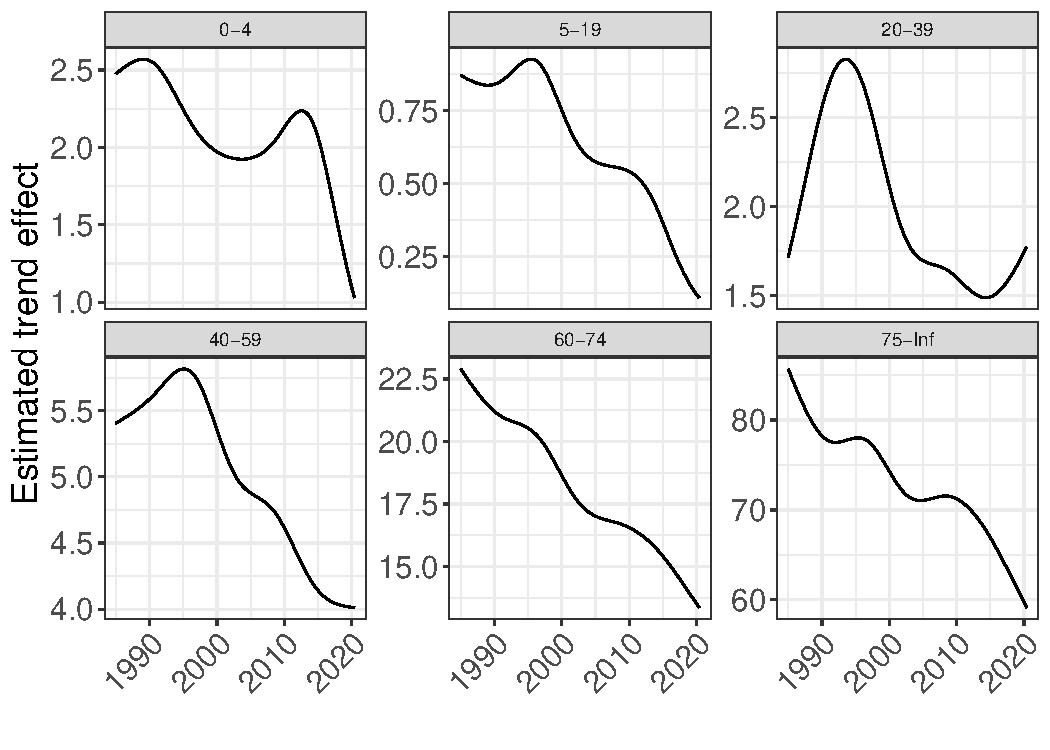
\includegraphics[width=1\linewidth]{figs/supp-figure-1a.pdf} 
	\end{subfigure}&
	\begin{subfigure}[t]{0.49\linewidth}
		\centering
		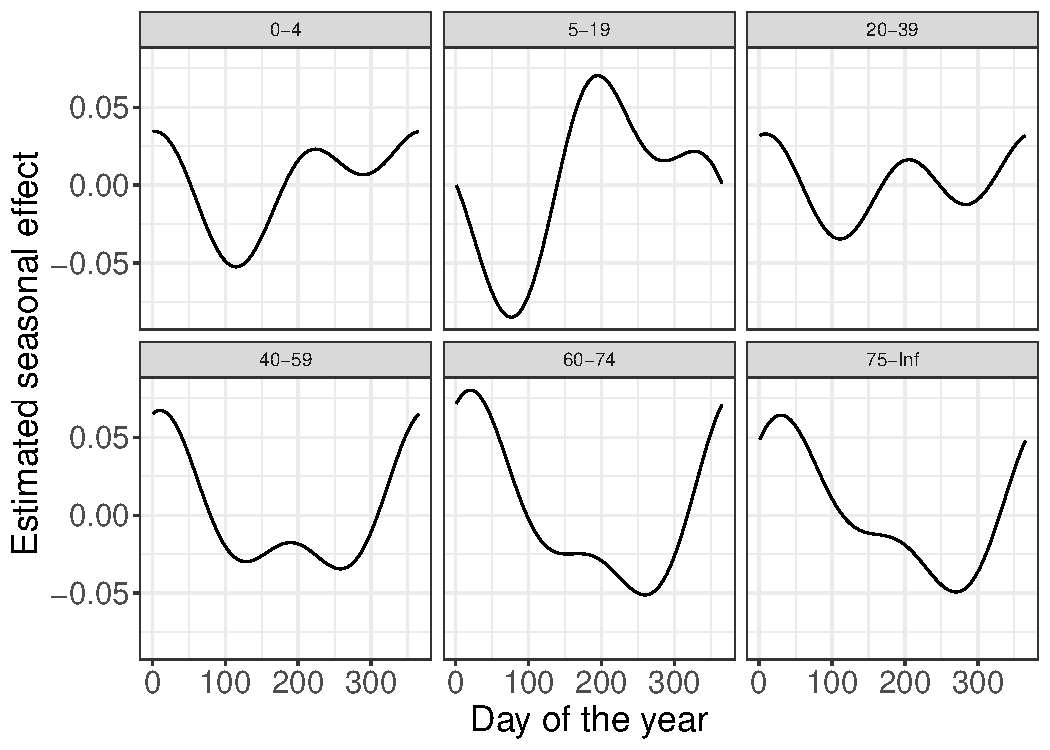
\includegraphics[width=1\linewidth]{figs/supp-figure-1b.pdf}
	\end{subfigure}&\\
    \end{tabular}
    \caption{Estimated components of the expected counts for six age groups in Puerto Rico. A) Death rate (deaths per 1,000 per year) trend components. B) Seasonal component for each age group as percentage increase or decrease from the average.}
    \label{supp-fig:model-components}
\end{suppfigure}

% Supp figure 2: F hat for all six hurricanes
\begin{suppfigure}[ht]
	\centering
	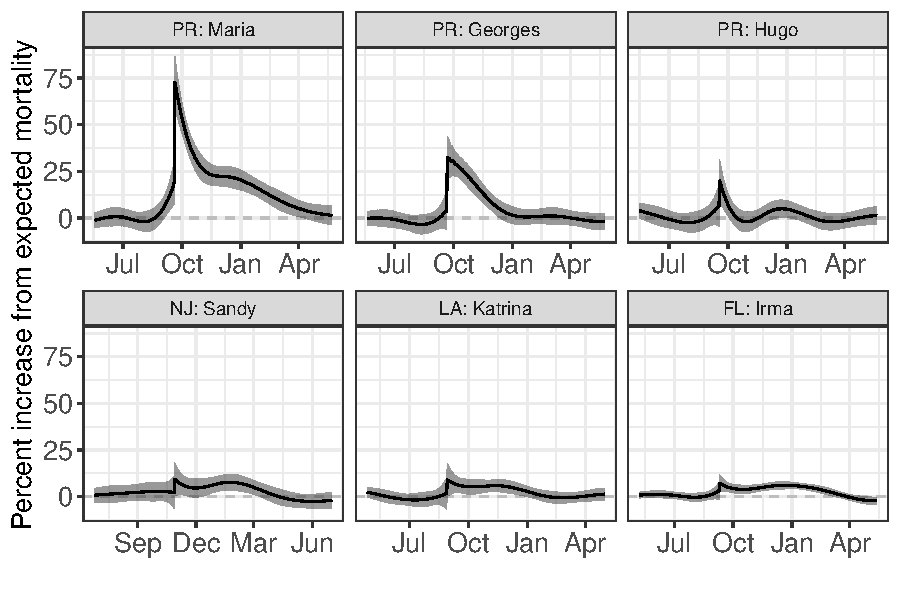
\includegraphics[width=1\linewidth]{figs/supp-figure-2.pdf} 
    \caption{Estimated hurricane effects as percent increase over expected mortality for the six hurricanes. The solid line corresponds to percent change from expected mortality and the shaded region represents a 95\% confidence interval.}
	\label{supp-fig:hurricane-effects}
\end{suppfigure}

% Supp figure 3: Fhat for age groups during chikungungya: NEED TO ADD FLU 2005
\begin{suppfigure}[ht]
	\centering
	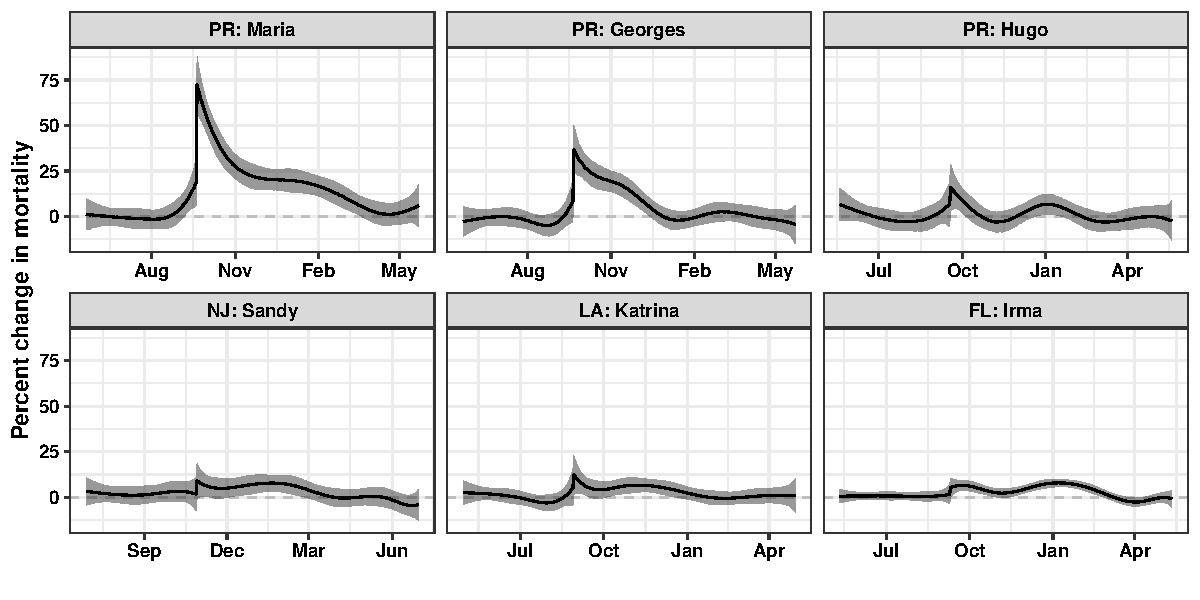
\includegraphics[width=1\linewidth]{figs/supp-figure-3.pdf} 
    \caption{Estimated event effects as percent increase over expected mortality. The solid line corresponds to percent change from expected mortality and the shaded region represents a 95\% confidence interval. A) Percent change during the Chikungunya epidemic in Puerto Rico for six age groups. B) Percent change during the 2005 flu season in Puerto Rico.}
	\label{supp-fig:chikungunya-agegroups}
\end{suppfigure}


% Supp figure 4: Top 12 jurisdiction most affected by covid 19 in USA
\begin{suppfigure}[ht]
	\centering
	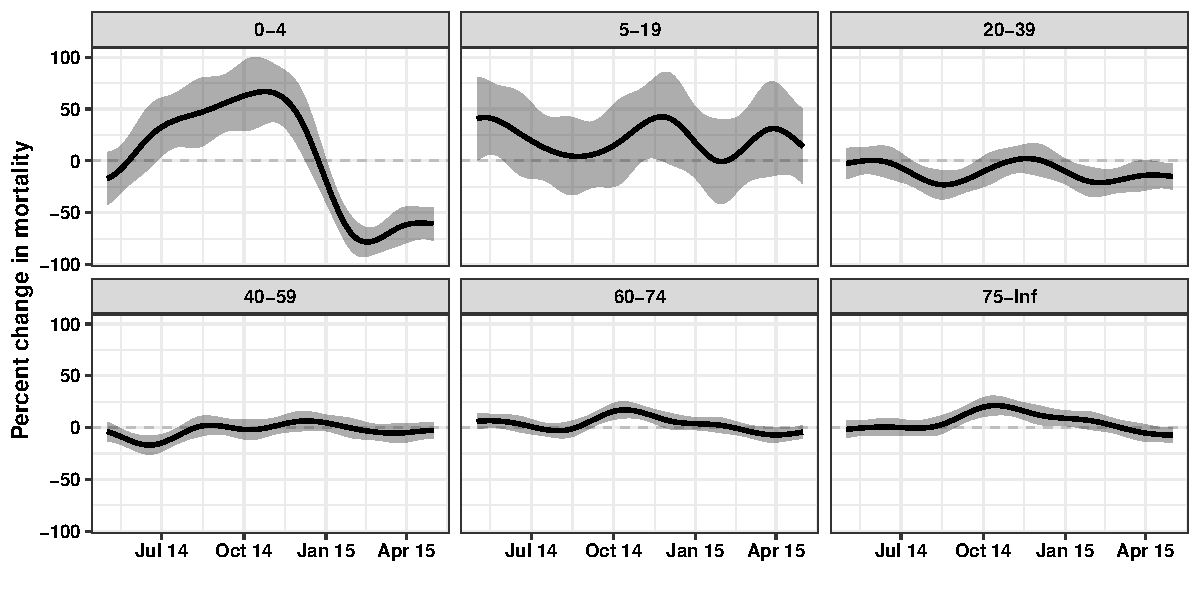
\includegraphics[width=1\linewidth]{figs/supp-figure-4.pdf} 
	\caption{Estimated event effects as percent increase over expected mortality for New York City and 8 states in the United States with the largest percent increase in mortality rates during the COVID-19 pandemic. The solid line corresponds to percent change from expected mortality and the shaded region represents a 95\% confidence interval. Note that no data was provided for Connecticut or North Carolina.}
	\label{supp-fig:covid19-states}
\end{suppfigure}

% Supp figure 6: Cook county effect by age groups
\begin{suppfigure}[ht]
	\centering
	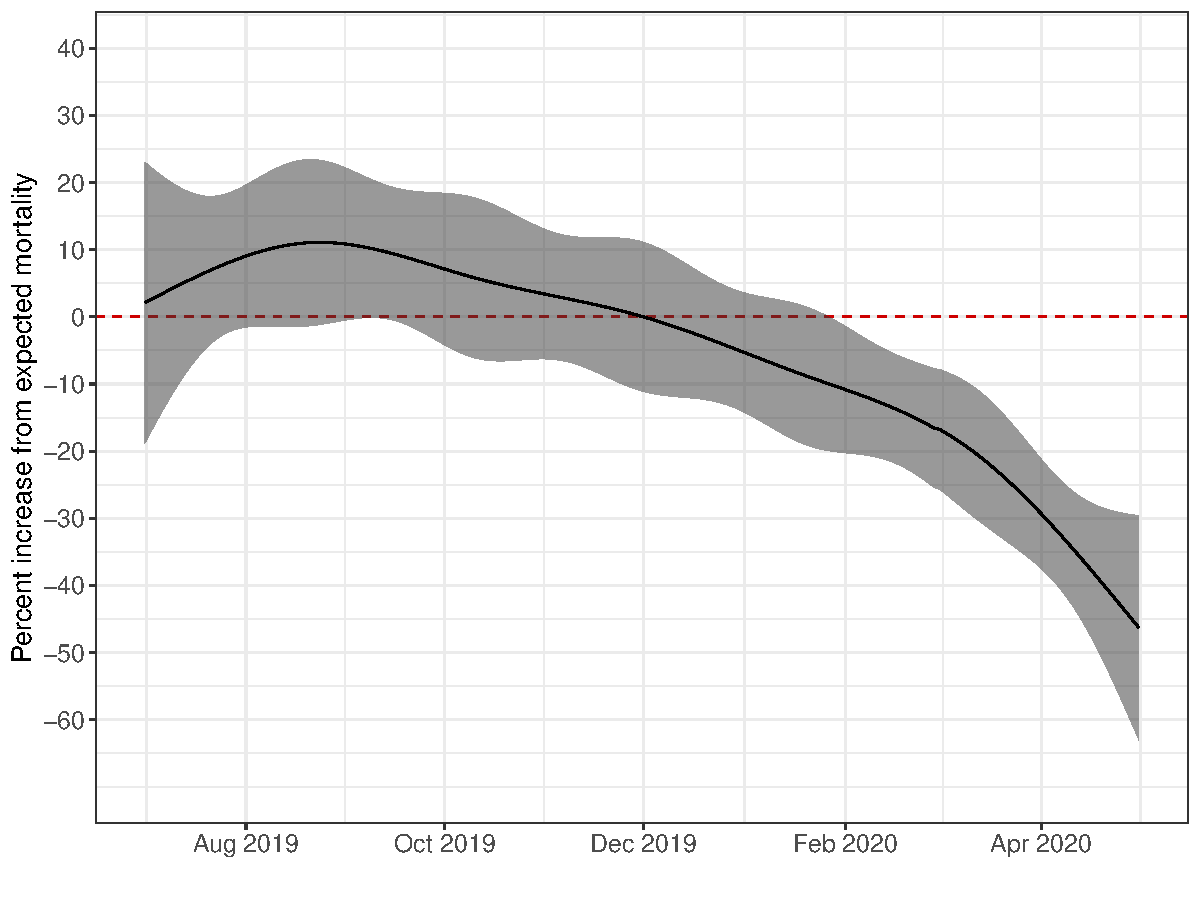
\includegraphics[width=1\linewidth]{figs/supp-figure-6.pdf} 
	\caption{Estimated effect of the COVID-19 pandemic in Cook county, IL, as percent increase over expected mortality stratified by age groups. The solid line corresponds to percent change from expected mortality and the shaded region represents a 95\% confidence interval.}
	\label{supp-fig:cook-agegroups}
\end{suppfigure}

% Supp figure 7: QQ plots and ACF
\begin{suppfigure}[ht]
	\begin{tabular}{lll}
	A&B\\
	\begin{subfigure}[t]{0.49\linewidth}
		\centering
		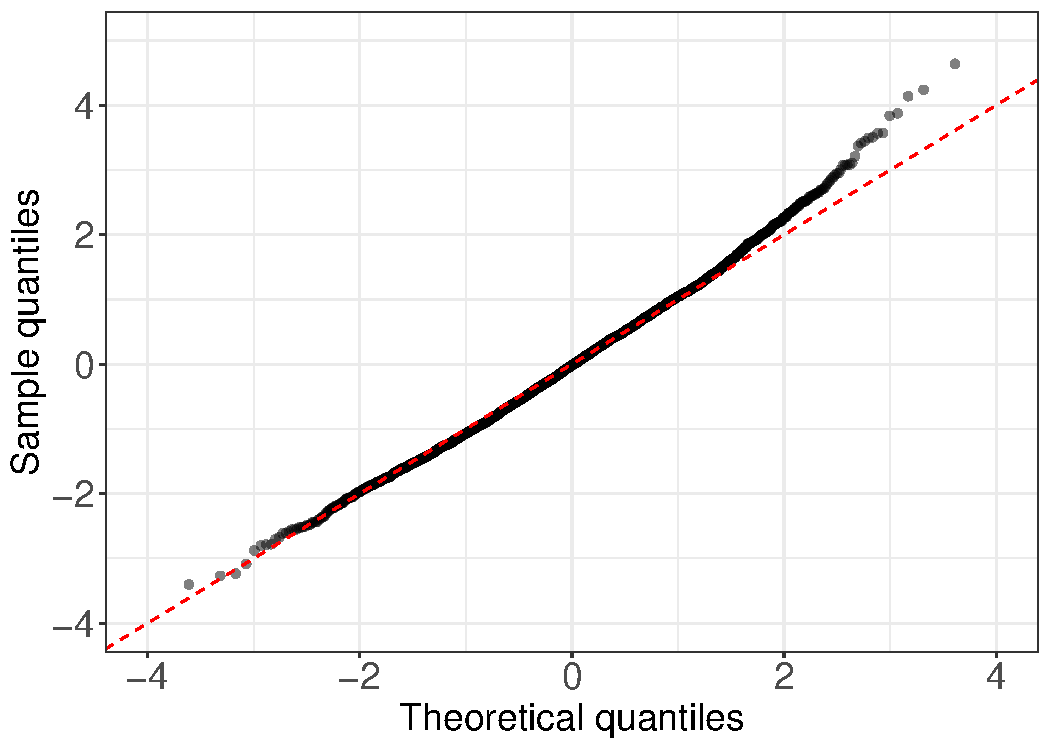
\includegraphics[width=1\linewidth]{figs/supp-figure-7a.pdf} 
	\end{subfigure}&
	\begin{subfigure}[t]{0.49\linewidth}
		\centering
		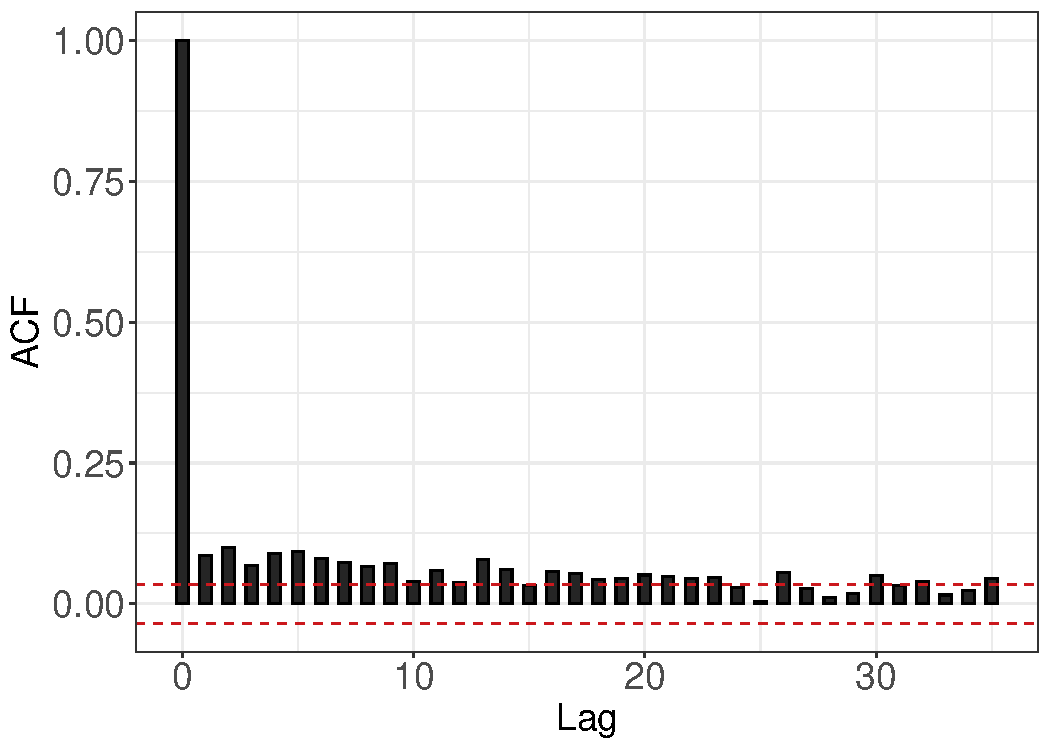
\includegraphics[width=1\linewidth]{figs/supp-figure-7b.pdf}
	\end{subfigure}&\\
	C&D\\
	\begin{subfigure}[t]{0.49\linewidth}
		\centering
		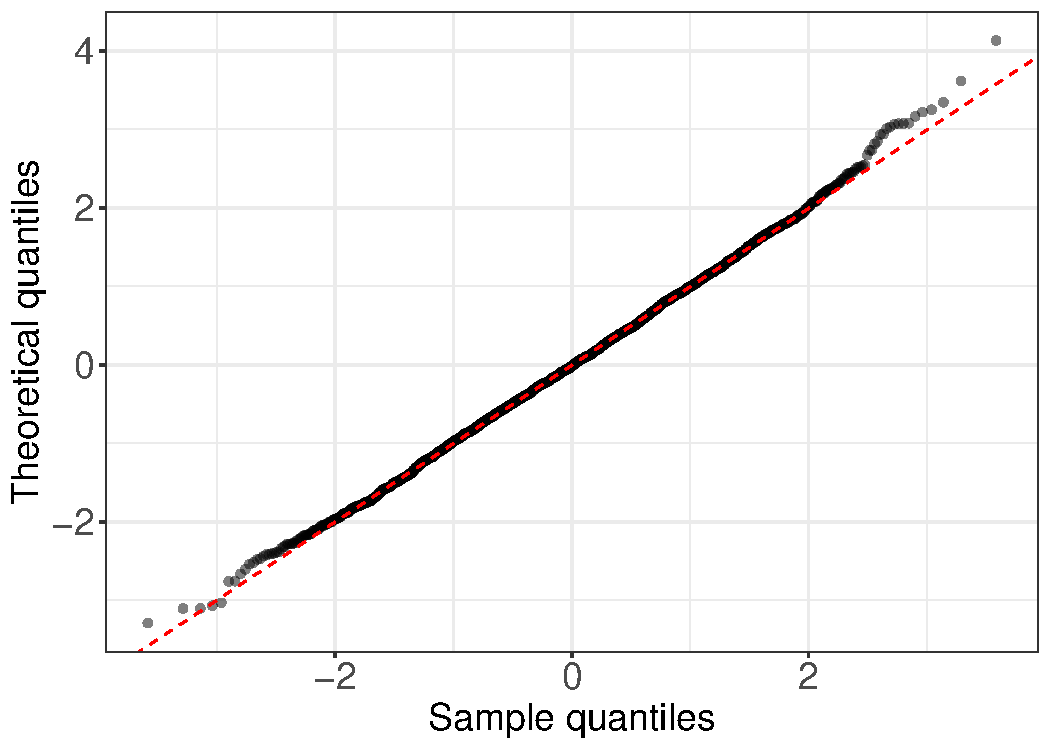
\includegraphics[width=1\linewidth]{figs/supp-figure-7c.pdf}
	\end{subfigure}&
	\begin{subfigure}[t]{0.49\linewidth}
    	\centering
	    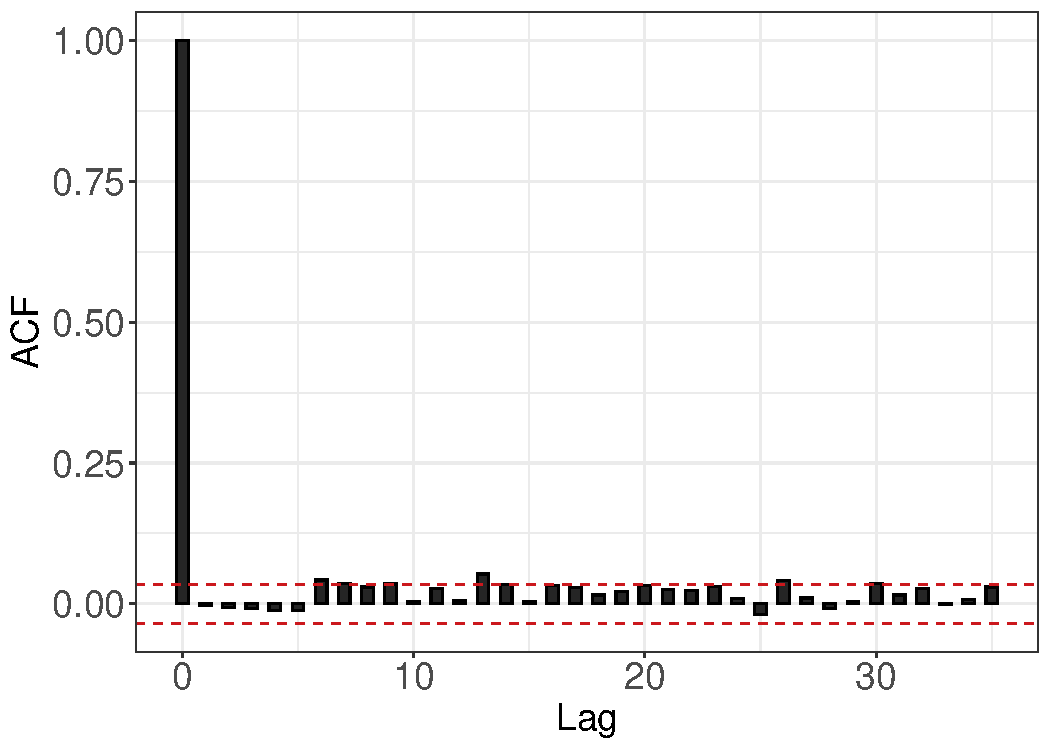
\includegraphics[width=1\linewidth]{figs/supp-figure-7d.pdf}
    \end{subfigure}\\
    \end{tabular}
    \caption{Evidence of correlated errors. A) A Poisson GLM was fitted to Puerto Rico daily death counts of individuals 75 years and over from an interval with no known natural disasters or outbreaks (Jan 1, 2006 to Dec 31, 2013). The plot shows the Pearson residuals quantiles versus theoretical quantiles from the normal distribution. One can see that the tail of the empirical data are larger than the theoretical values. B) The sample autocorrelation function for these Pearson residuals with the red-dash lines represent a 95\% confidence interval centered at zero. C) As A) but for residuals after prewhitening based on an estimate of the covariance matrix. D) As B) but for the prewhittened residuals.}
    \label{supp-fig:correlated-errors}
\end{suppfigure}

% Supp figure 8: Population displacement in Puerto Rico
\begin{suppfigure}[ht]
	\centering
	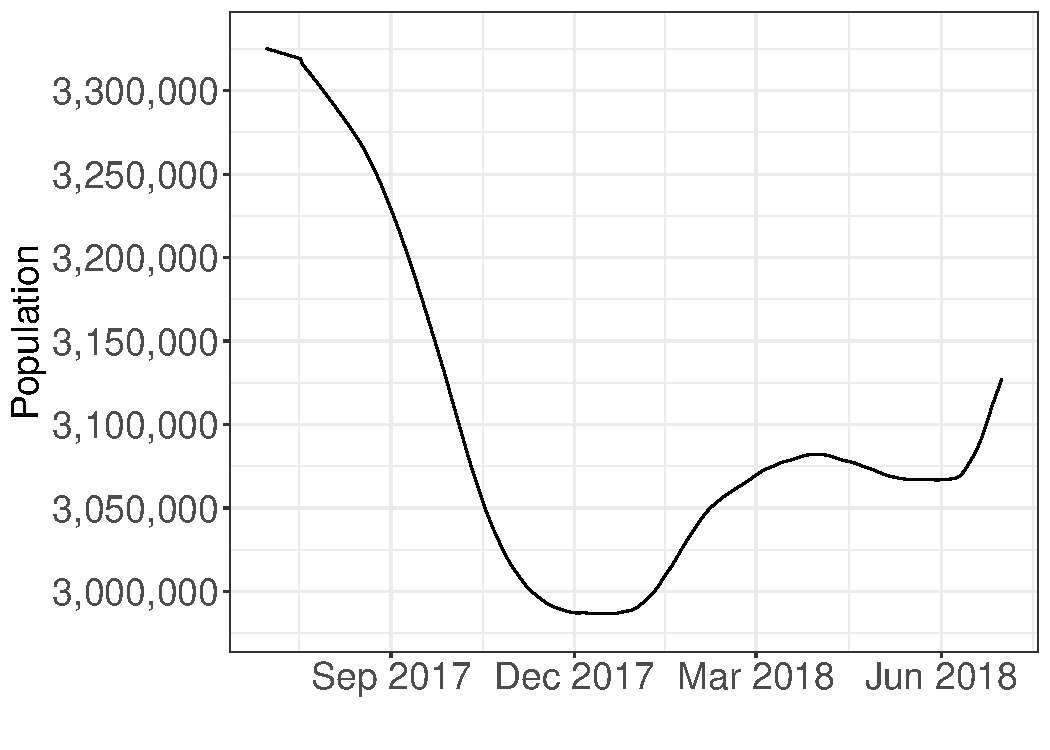
\includegraphics[width=0.70\linewidth]{figs/supp-figure-8.pdf} 
	\caption{Estimated population displacement in Puerto Rico after Hurricane Mar\'ia.}
	\label{supp-fig:pop-displacement-pr}
\end{suppfigure}


% Supp figure 9: Model comparison with weekly data
\begin{suppfigure}[ht]
	\begin{tabular}{lll}
	A&B&C\\
	\begin{subfigure}[t]{0.30\linewidth}
		\centering
		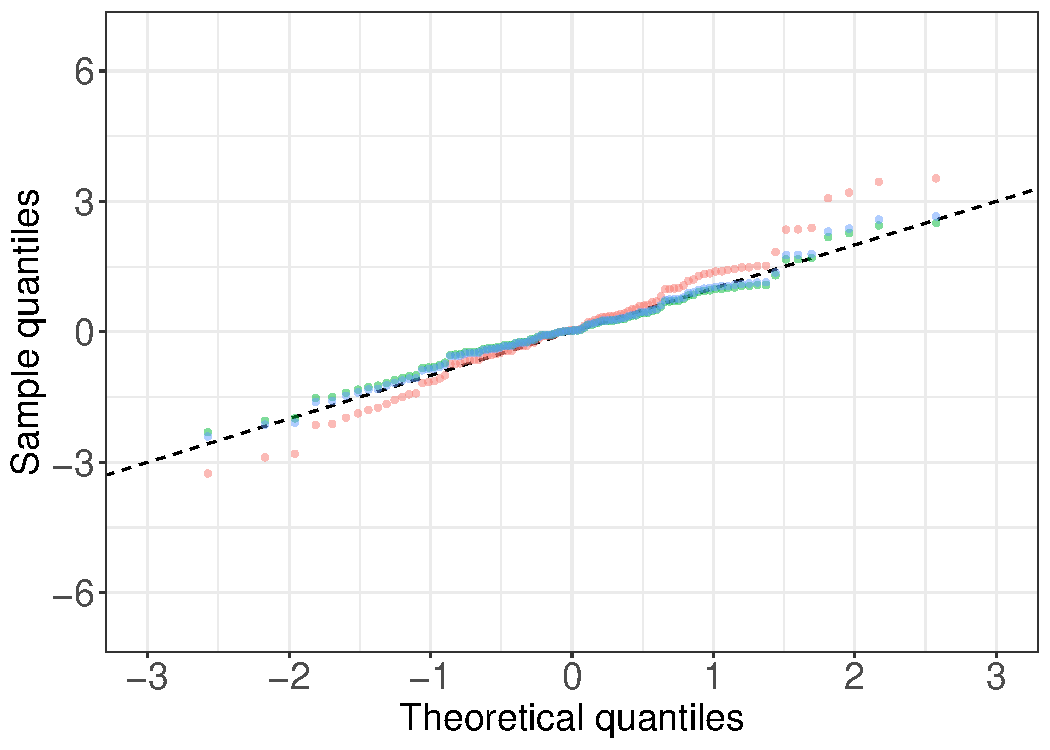
\includegraphics[width=1\linewidth]{figs/supp-figure-9a.pdf} 
	\end{subfigure}&
	\begin{subfigure}[t]{0.30\linewidth}
		\centering
		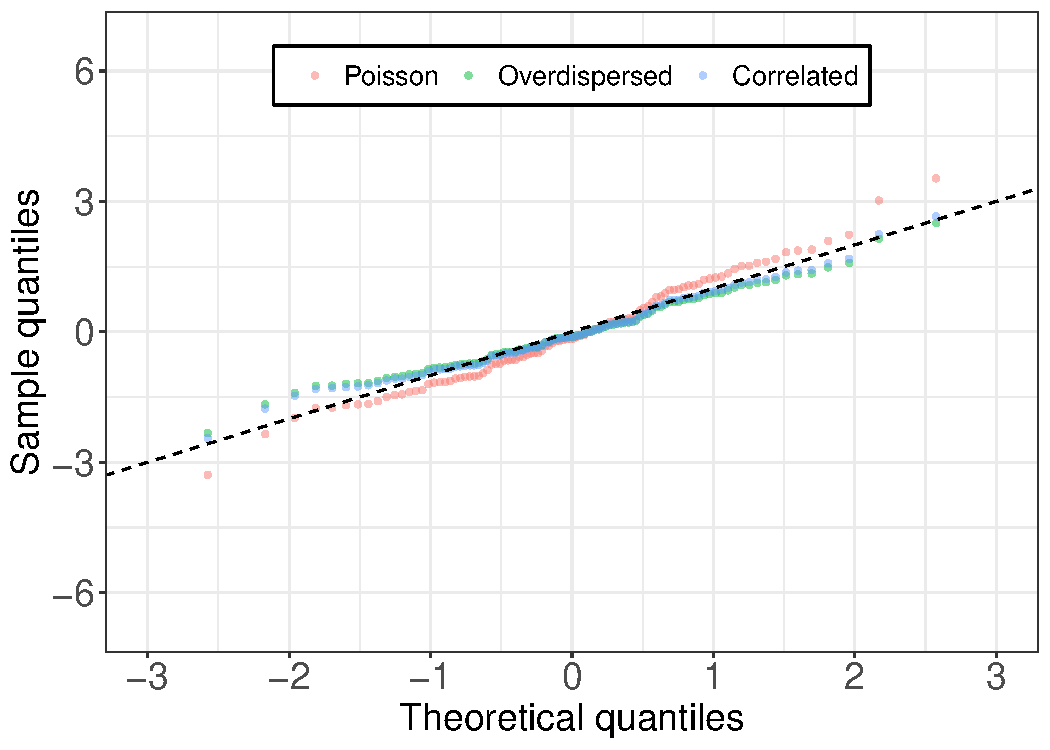
\includegraphics[width=1\linewidth]{figs/supp-figure-9b.pdf}
	\end{subfigure}&
	\begin{subfigure}[t]{0.30\linewidth}
		\centering
		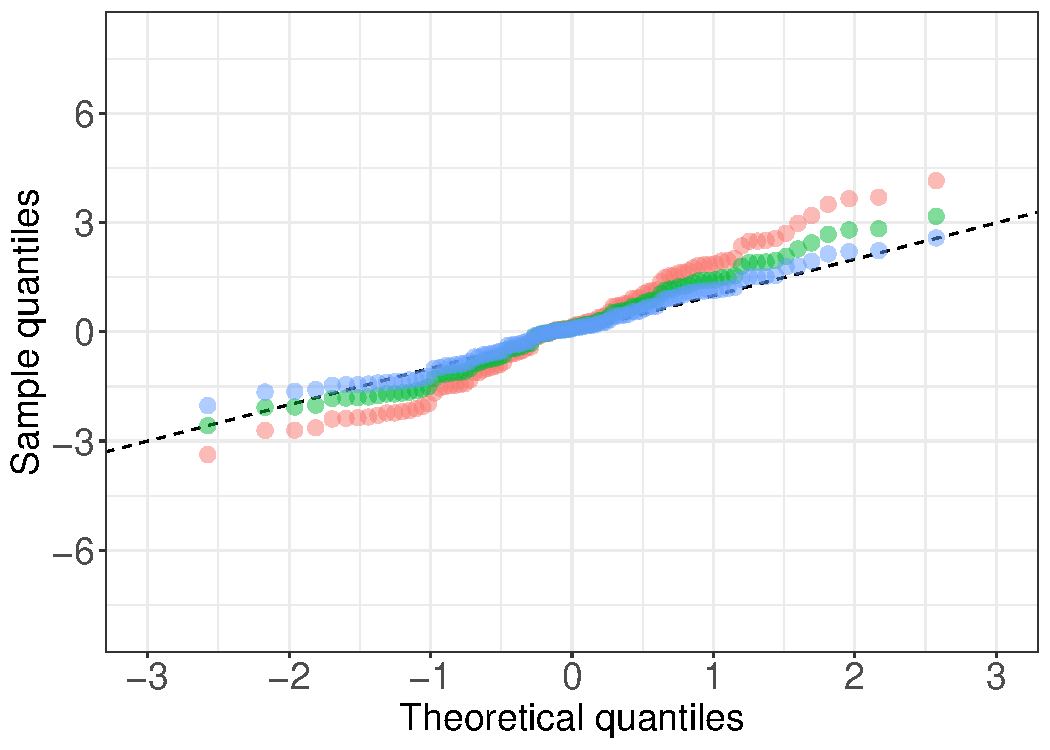
\includegraphics[width=1\linewidth]{figs/supp-figure-9c.pdf}
	\end{subfigure}\\
    \end{tabular}
    \caption{Accounting for correlation in the error structure of weekly data yields very similar uncertainty estimates to over-dispersed Poisson GLM. We fitted our model along with a Poisson and over-dispersed Poisson GLM to weekly Puerto Rico mortality data of individuals 75 years and over, and randomly picked 100 intervals of varying sizes to compute z-scores of total number of deaths. Each plot shows the Pearson residual quantiles versus theoretical quantiles from the standard normal distribution. A) Intervals of 1 week. B) Intervals of 7 weeks. C) Intervals of 14 weeks.}
    \label{supp-fig:weekly-correlated}
\end{suppfigure}

% Supp figure 10: Simulation study
\begin{suppfigure}[ht]
	\begin{tabular}{lll}
	A&B&C\\
	\begin{subfigure}[t]{0.30\linewidth}
		\centering
		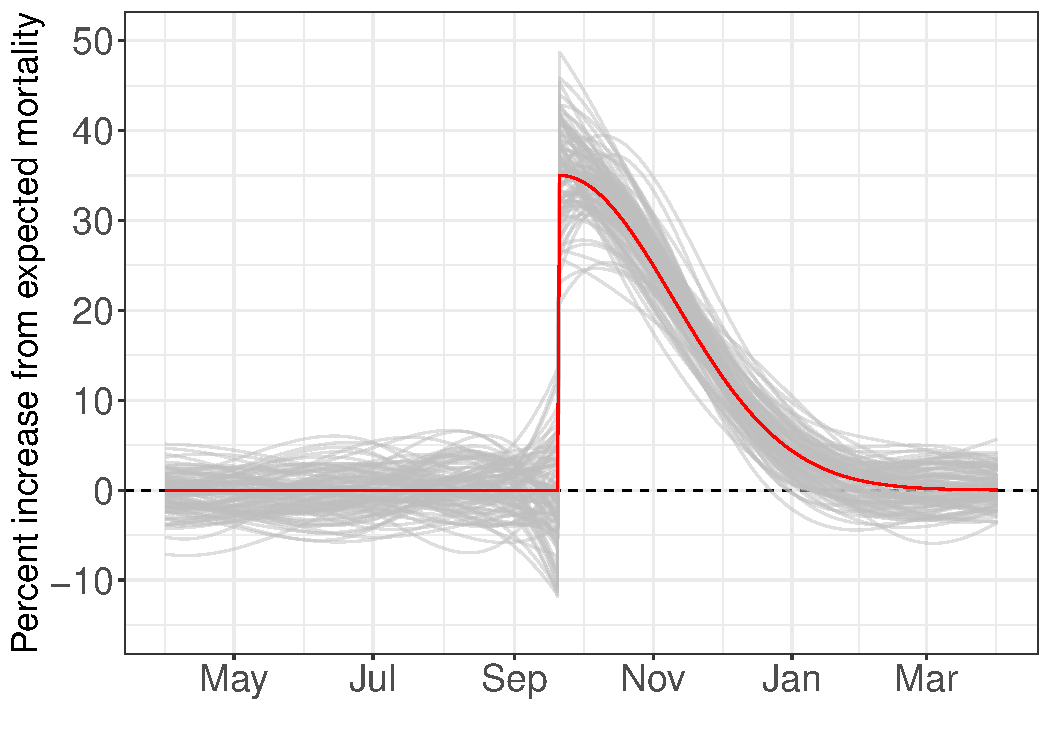
\includegraphics[width=1\linewidth]{figs/supp-figure-10a.pdf} 
	\end{subfigure}&
	\begin{subfigure}[t]{0.30\linewidth}
		\centering
		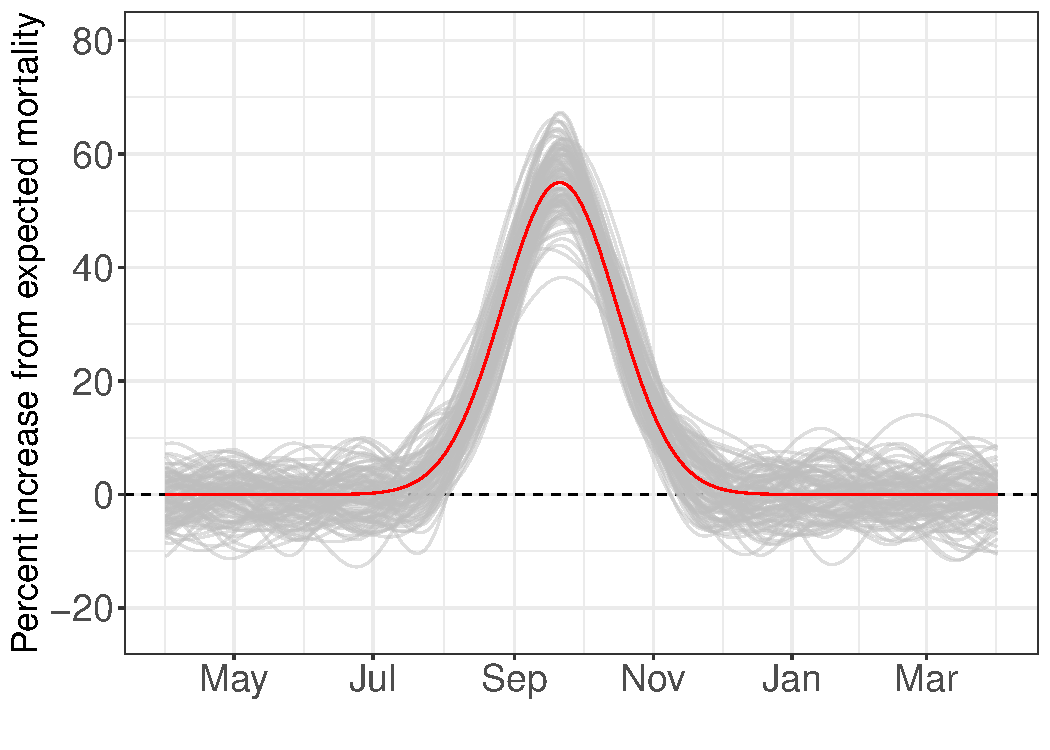
\includegraphics[width=1\linewidth]{figs/supp-figure-10b.pdf}
	\end{subfigure}&
	\begin{subfigure}[t]{0.30\linewidth}
		\centering
		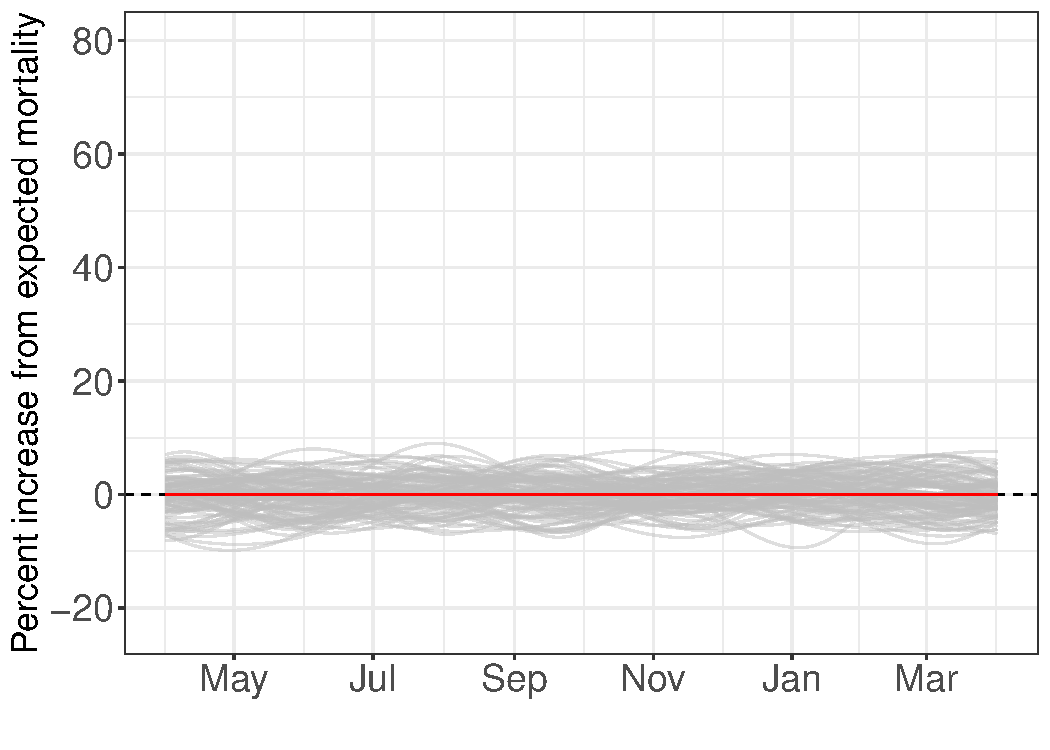
\includegraphics[width=1\linewidth]{figs/supp-figure-10c.pdf}
	\end{subfigure}\\
	D&E&F\\
	\begin{subfigure}[t]{0.30\linewidth}
		\centering
		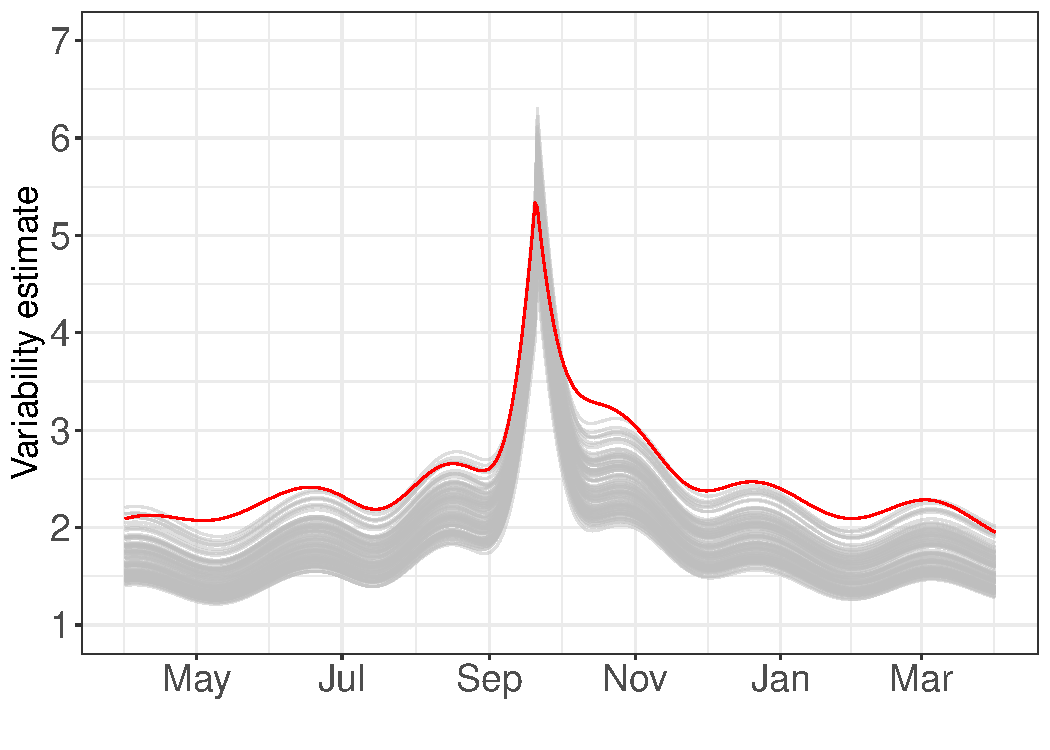
\includegraphics[width=1\linewidth]{figs/supp-figure-10d.pdf} 
	\end{subfigure}&
	\begin{subfigure}[t]{0.30\linewidth}
		\centering
		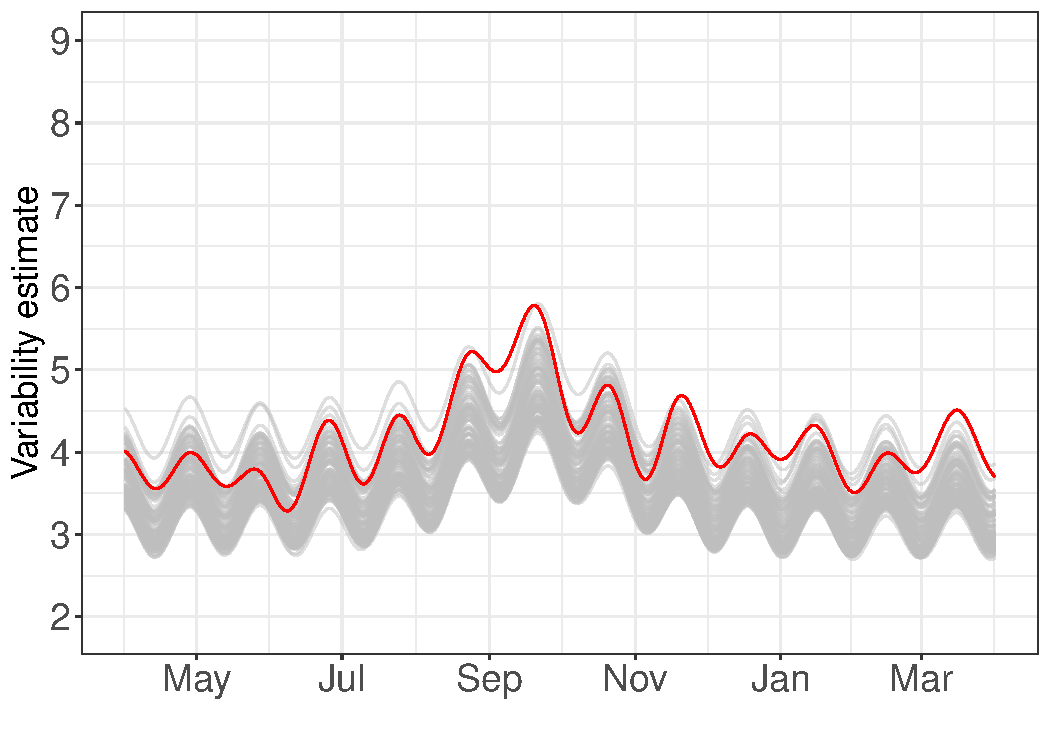
\includegraphics[width=1\linewidth]{figs/supp-figure-10e.pdf}
	\end{subfigure}&
	\begin{subfigure}[t]{0.30\linewidth}
		\centering
		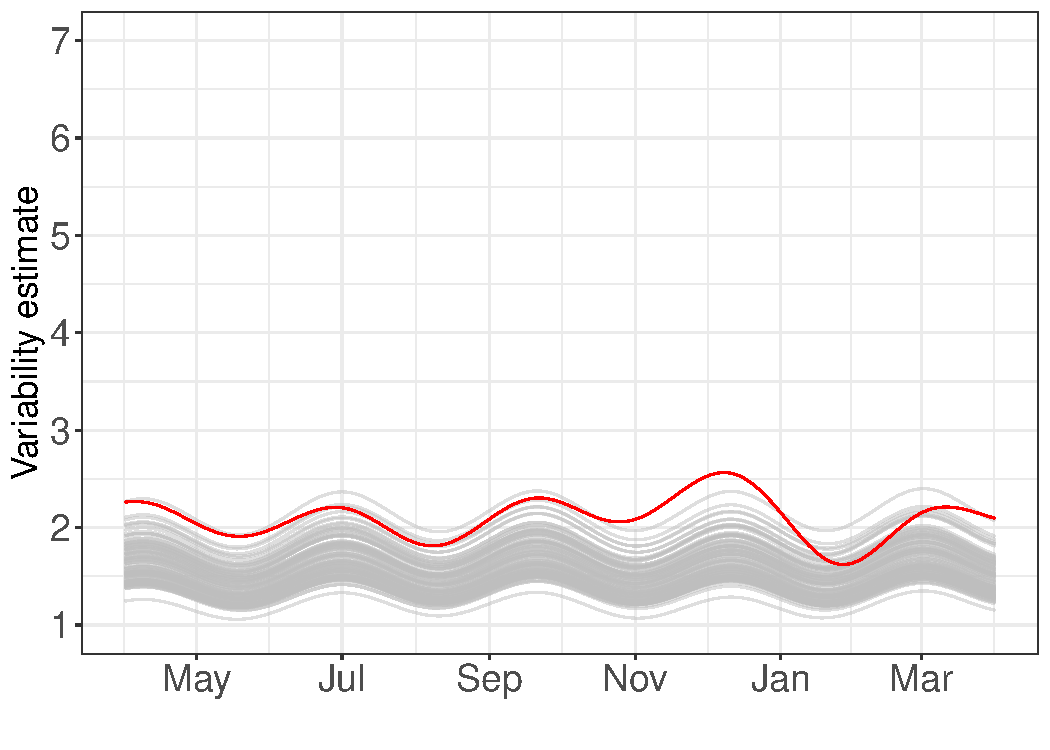
\includegraphics[width=1\linewidth]{figs/supp-figure-10f.pdf}
	\end{subfigure}\\
    \end{tabular}
    \caption{Simulation study. For all three scenarios, the event day $(t_0)$, the effect size $(\theta)$, and the period of effect $(L)$ are September 21, 1998, 55\%, and 150 days, respectively. For each scenario we ran 100 simulations. A) Percent increase in mortality from the average in the hypothetical scenario of a hurricane making landfall on September 21, 1998. The gray lines correspond to estimates from each simulation and the red line represents the true curve. B) Percent increase in mortality from the average in the hypothetical scenario of an epidemic with peak mortality on September 21, 1998. The gray lines correspond to estimates from each simulation and the red line represents the true curve. C) Percent change from expected mortality during a period with no event. D), E), and F) Estimated standard error of $\hat{f}(t)$ for each scenario, respectively. The gray lines correspond to the standard error estimates for each simulation and the red line represents the true standard error, estimated from the simulation.}
    \label{supp-fig:simulations}
\end{suppfigure}
\end{document}